\chapter{Weighted Directional Total Nuclear Variation for Joint $^{90}$Y PET/SPECT Reconstruction with CTAC-derived Guidance}
\label{chapter:paper}

This chapter applies the \acrfull{wdtnv} prior developed in Chapter~\ref{chapter:wdtnv} to the clinically relevant problem of post-treatment $^{90}$Y activity imaging after \glsentryshort{sirt}. We consider joint reconstruction of low-count $^{90}$Y \glsentryshort{pet} and bremsstrahlung \glsentryshort{spect}, using \acrfull{ctac} information directionally (via the \glsentryshort{ctac}-derived attenuation map $\mu$).

Building on the single-bed phantom optimisation study in Chapter~\ref{chapter:optimisation}, we extend the reconstruction framework to multiple PET bed positions for patient imaging. The focus here is validation and comparison with other methods: we specify modality-dependent forward models, co-registration operators, practical normalisation for heterogeneous \glsentryshort{pet}/\glsentryshort{spect} scales, and a reproducible evaluation protocol on a \acrfull{nema} \acrfull{iec} phantom with \glsentryshort{pet} bootstrapping and on a post-\glsentryshort{sirt} patient cohort.

\section{Motivation and clinical context}
\label{sec:90y_motivation}

Quantitative post-treatment imaging is required for personalised dosimetry following $^{90}$Y \glsentryshort{sirt} \cite{levillainInternationalRecommendationsPersonalised2021}. Pre-treatment planning based on $^{99\mathrm{m}}$Tc-\gls{maa} often mis-predicts microsphere deposition, motivating post-treatment verification of delivered activity distributions \cite{hasteCorrelationTechnetium99mMacroaggregated2017}.

Two $^{90}$Y modalities are clinically available:
\begin{itemize}
    \item \textbf{$^{90}$Y PET}: detects the rare internal pair-production branch, providing comparatively high spatial resolution but extremely low count statistics \cite{selwynNewInternalPair2007}.
    \item \textbf{Bremsstrahlung SPECT}: has substantially higher corrected counts (about $15\times$ for the data studied here) but suffers from severe blur, septal penetration, and scatter due to the continuous emission spectrum \cite{rongDevelopmentEvaluationImproved2012, minarikEvaluationQuantitative90Y2008}.
\end{itemize}
Both modalities are typically acquired alongside CT for attenuation correction and anatomical localisation. Since PET and SPECT image the same underlying microsphere distribution while CTAC provides structural rather than activity information, independent reconstruction discards both a strong physical coupling and useful anatomical context.

The \gls{shkem} method of Deidda \textit{et al.} improves lesion contrast by reconstructing one modality to guide another \cite{deiddaTripleModalityImage2023, deiddaHybridKernelisedExpectation2022}. However, this method remains sensitive to iteration choice and noise amplification. This motivates a truly joint MAP formulation with a coupled regulariser that promotes shared geometry while allowing modality-specific contrast.

\section{Joint MAP formulation for PET/SPECT}
\label{sec:90y_joint_map}

We use the joint MAP framework introduced in Section~\ref{subsec:synergistic_recon}. For the present application we set $M=2$ modalities, with $m=1$ denoting PET and $m=2$ denoting SPECT\@. Let $z_m\in\mathbb{R}_+^{N}$ denote the image for modality $m$ represented on a shared grid and let $y_m\in\mathbb{N}^{I_m}$ denote the corresponding projection data.

The native image grid for modality $m$ may differ from the shared grid. Let $W_m:\mathbb{R}_+^{J_m}\to\mathbb{R}_+^{N}$ denote the discrete resampling operator from the native grid to the shared grid, and let $W_m^\ast:\mathbb{R}_+^{N}\to\mathbb{R}_+^{J_m}$ denote its discrete adjoint. The adjoint maps shared-grid variables back to the native grid before application of the system matrix. For each modality we therefore use the affine Poisson model
\begin{equation}
\bar y_m(z_m) = A_m W_m^\ast z_m + b_m,
\end{equation}
where $A_m$ is the system matrix and $b_m$ collects additive corrections. For example, randoms and scatter for PET and simulated scatter/penetration terms for SPECT (see Sections~\ref{subsec:90y_pet_forward} and~\ref{subsec:90y_spect_forward}).

The joint objective is
\begin{equation}
\hat{\bm{z}}
=
\arg\min_{\bm{z}\ge 0}
\left\{
\sum_{m=1}^{2}\mathcal{D}_m\!\left(y_m \mid A_m W_m^\ast z_m + b_m\right)
+
\widetilde{\mathcal{R}}(\bm{z})
\right\},
\label{eq:90y_joint_obj}
\end{equation}
where $\mathcal{D}_m$ is the Poisson negative log-likelihood (up to an additive constant),
\begin{equation}
\mathcal{D}_m(y_m\mid \bar y_m)=\sum_{i=1}^{I_m}\left((\bar y_m)_i - (y_m)_i\log (\bar y_m)_i\right),
\end{equation}
and $\widetilde{\mathcal{R}}$ is the coupled prior. Throughout this thesis, a tilde on a TV- or TNV-type regularisation functional denotes its smoothed version. Thus $\widetilde{\mathcal{R}}$ is the smoothed $w$-$d$TNV prior $\widetilde{\mathcal{R}}_{\mathrm{w\text{-}dTNV}}$ defined in Section~\ref{sec:wdtnv} (Chapter~\ref{chapter:wdtnv}). The overall regularisation strength is carried by the modality weights introduced below, so no separate global scalar prior multiplier is used in the implementation.

\subsection{Multi-Bed \gls{pet} Acquisition}
\label{sec:multibed}

The patient acquisitions in this chapter use two partially overlapping \gls{pet} bed positions to extend the axial coverage beyond a single field of view. Structures of interest can therefore extend into the low-sensitivity edge of an individual bed, while two beds contribute measurements of the shared anatomy in their overlap. A coupled edge-preserving prior ideally should act on one activity field spanning the whole acquisition, rather than on images divided by scanner bed boundaries.

\subsubsection{Why Not Stitch Independent Reconstructions?}
\label{subsec:stitching_failure}

A common practical alternative is to reconstruct each \gls{pet} bed independently and fuse the images using sensitivity-weighted stitching in the overlap. With an edge-preserving prior, however, each reconstruction makes its own noise-suppression and edge decisions before fusion. We performed a qualitative comparison between this post-reconstruction fusing and the joint multi-bed formulation described below \cite{porterSimultaneousMultiBedMAP2025}. Figure~\ref{fig:optim_multibed_qualitative} shows overlap-region noise and discontinuities after separate reconstruction and fusion.

\begin{figure}[htbp]
    \centering
    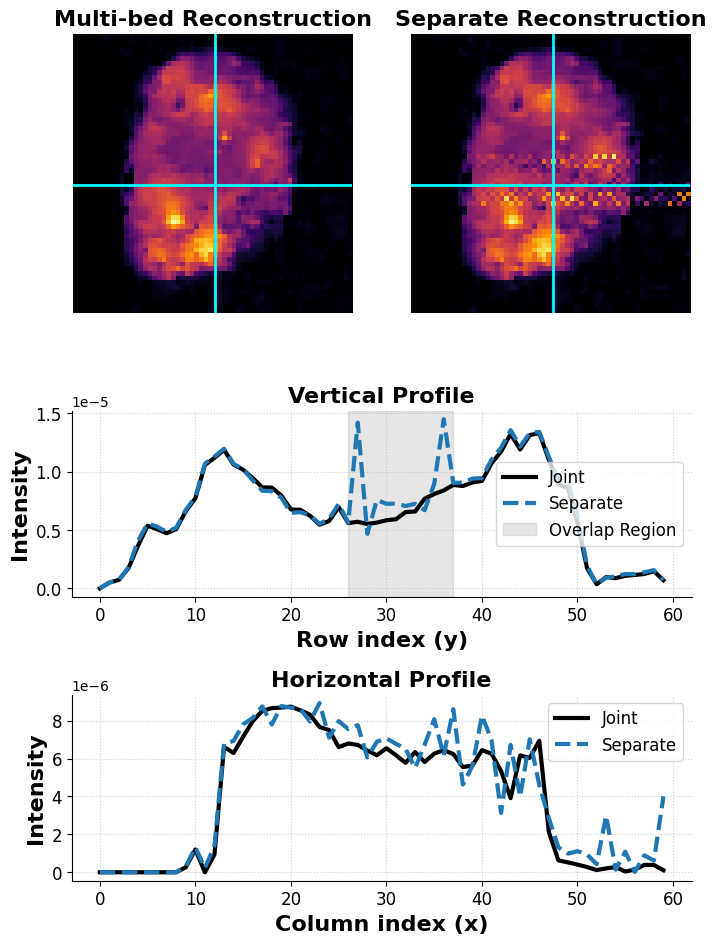
\includegraphics[width=0.72\linewidth]{figures/PiW/comparison.png}
    \caption{Qualitative comparison of separately reconstructed and fused \gls{pet} bed positions with a joint multi-bed reconstruction using \gls{ct}-guided edge-preserving regularisation (from \cite{porterSimultaneousMultiBedMAP2025}). The shaded region marks the bed overlap and the cyan lines mark the displayed profiles.}
    \label{fig:optim_multibed_qualitative}
\end{figure}

\subsubsection{Joint Multi-Bed Formulation}
\label{subsec:multibed_notation}
\label{subsec:joint_multibed}

Let $z_1$ be the \gls{pet} activity image on the combined shared reconstruction grid. For bed position $\mathrm{p}=1,\ldots,N_{\mathrm{p}}$, let $R_{\mathrm{p}}$ restrict the combined image to the axial support reconstructed by that bed. The expected \gls{pet} data for bed position $\mathrm{p}$ are
\begin{equation}
    \bar y_{\mathrm{p}}(z_1)
    =
    A_{\mathrm{p}} R_{\mathrm{p}} z_1 + b_{\mathrm{p}},
    \label{eq:multibed_forward_model}
\end{equation}
where $A_{\mathrm{p}}$ is the bed-specific \gls{pet} system matrix and $b_{\mathrm{p}}$ collects additive corrections. The joint \gls{pet} data term is
\begin{equation}
    \mathcal{D}_{\mathrm{PET}}^{\mathrm{multi}}(z_1)
    =
    \sum_{\mathrm{p}=1}^{N_{\mathrm{p}}}
    \mathcal{D}
    \left(
        y_{\mathrm{p}} \mid A_{\mathrm{p}} R_{\mathrm{p}} z_1 + b_{\mathrm{p}}
    \right),
    \label{eq:multibed_data_term}
\end{equation}
with gradient
\begin{equation}
    \nabla \mathcal{D}_{\mathrm{PET}}^{\mathrm{multi}}(z_1)
    =
    \sum_{\mathrm{p}=1}^{N_{\mathrm{p}}}
    R_{\mathrm{p}}^\top
    A_{\mathrm{p}}^\top
    \nabla_{\bar y_{\mathrm{p}}}
    \mathcal{D}
    \left(
        y_{\mathrm{p}} \mid A_{\mathrm{p}} R_{\mathrm{p}} z_1 + b_{\mathrm{p}}
    \right).
    \label{eq:multibed_gradient}
\end{equation}
The corresponding \gls{pet} sensitivity image on the combined grid is
\begin{equation}
    s_{\mathrm{PET}}^{\mathrm{multi}}
    =
    \sum_{\mathrm{p}=1}^{N_{\mathrm{p}}}
    R_{\mathrm{p}}^\top A_{\mathrm{p}}^\top \bm 1.
    \label{eq:multibed_sensitivity}
\end{equation}
Each bed contributes its own data term and sensitivity to a single combined image, while the image-domain prior is evaluated over the complete field of view. For the joint PET/SPECT objective~\eqref{eq:90y_joint_obj}, $\mathcal{D}_1$ is replaced by the summed multi-bed PET data term~\eqref{eq:multibed_data_term}; the SPECT data term and coupled prior retain their existing form. Likewise, the PET sensitivity used for preconditioning is the combined sensitivity~\eqref{eq:multibed_sensitivity}. This extends the single-bed optimisation framework tested in Chapter~\ref{chapter:optimisation} to the two-bed patient acquisitions evaluated here.

\section{$w$-$d$TNV for $^{90}$Y PET/SPECT with CTAC guidance}
\label{sec:90y_wdtnv}

\subsection{Directional guidance from the CTAC-derived $\mu$-map}
\label{subsec:90y_mu_guidance}

We apply the directional construction in~\eqref{eq:wdtnv_directional_operator} using the CTAC-derived attenuation map $\mu$ as the guidance image, resampled to the shared \gls{pet} grid. We pre-smooth $\mu$ with a blurring kernel ($\mathrm{FWHM}=\SI{2}{\milli\metre}$) to reduce high-frequency CT noise while retaining high guidance edge resolution. The direction field $\xi_n$ is computed with the empirical stabiliser
\begin{equation}
\eta = 0.05\cdot \max_{n}\|(D\mu)_n\|_2,
\label{eq:90y_xi_def}
\end{equation}
where $D$ is specified in Section~\ref{subsec:90y_directional_stencil}. Unless stated otherwise, the directional operators use $\gamma_1=\gamma_2=1$.

\subsection{Global modality normalisation}
\label{subsec:90y_global_weights}

We specialise the modality weighting from~\eqref{eq:Bn_def} to a spatially uniform normalisation to mitigate the dominant scale disparity between $^{90}$Y PET and bremsstrahlung SPECT:
\begin{equation}
B_n \equiv B := \mathrm{diag}(\rho_1,\rho_2),
\qquad \rho_1,\rho_2>0.
\end{equation}
Weights are computed from early-stopped unregularised reconstructions represented on the shared grid, $z_m^{\mathrm{init}}$, via dynamic-range (percentile) scaling over a CTAC-derived foreground mask $\Omega'$:
\begin{equation}
\rho_m
=
\frac{\beta_m}{q_{0.99}\!\bigl(z_m^{\mathrm{init}}|_{\Omega'}\bigr)-q_{0.01}\!\bigl(z_m^{\mathrm{init}}|_{\Omega'}\bigr)},
\qquad m\in\{1,2\},
\label{eq:90y_rhom_def}
\end{equation}
where $q_p(\cdot|_{\Omega'})$ denotes the $p$-quantile (so $q_{0.01}$ and $q_{0.99}$ are the 1st and 99th percentiles) over voxels in $\Omega'$, and $\beta_m$ are user-controlled regularisation weights used for operating-point selection (Section~\ref{subsec:90y_hyperparams}). Thus $\beta_m$ is the chosen modality-specific regularisation setting, whereas $\rho_m$ is the resulting weight applied to the modality gradient after intensity normalisation. Here $\rho_{m,n}=\rho_m$ for every voxel $n$. The regularisation settings enter the prior through these weights, so the objective uses no additional global multiplier $\beta$. Percentile scaling provides a robust dynamic-range estimate and reduces sensitivity to outliers. This matches the intent of Section~\ref{subsec:modality_weighting} while avoiding an additional spatially varying weight for this investigation \cite{tsaiBenefitsUsingSpatiallyVariant2020}.

\subsection{Directional finite-difference operator for PET/SPECT coupling}
\label{subsec:90y_directional_stencil}

We specialise the finite-difference operator from~\eqref{eq:finite_difference} with offsets chosen to better accommodate SPECT blur and modest registration error. Let $\Delta=(\Delta_x,\Delta_y,\Delta_z)$ denote the voxel sizes in SI units. We define a nine-direction half-stencil
\begin{equation}
\mathcal{E}_1
=
\{(1,0,0),(0,1,0),(0,0,1)\}
\cup
\{(\pm1,1,0),(\pm1,0,1),(0,1,\pm1)\},
\end{equation}
and use both one- and two-voxel steps, $\mathcal{E}=\mathcal{E}_1\cup\{2e:e\in\mathcal{E}_1\}$, yielding $d=18$ directions. For a set of offsets $\mathcal{E}=\{e_\ell\}_{\ell=1}^{d}$, define the $d$-directional forward difference operator $D$ by
\begin{equation}
\big((D z)_n\big)^{(\ell)} :=
\frac{z_{n+e_\ell}-z_n}{\|e_\ell\|_\Delta},
\qquad
\|e\|_\Delta := \sqrt{(e_x\Delta_x)^2+(e_y\Delta_y)^2+(e_z\Delta_z)^2},
\label{eq:90y_directional_D}
\end{equation}
with Neumann boundary conditions. This follows the ``extended Jacobian'' motivation for TNV-type coupling \cite{holtTotalNuclearVariation2014} and empirically improved stability in the present PET/SPECT setting.

\subsection{Smoothing parameter}
\label{subsec:90y_wdtnv_def}

The weighted directional Jacobian and regulariser follow Equations~\eqref{eq:Yn_weighted} and~\eqref{eq:wdtnv_prior}, with $z_1$ representing PET and $z_2$ representing SPECT. We set the smoothing parameter $\epsilon$ relative to initial joint-gradient magnitudes, using the square root of the largest Gram eigenvalue:
\begin{equation}
\epsilon
=
0.05\cdot \mathrm{median}_{n\in\Omega'}\,\sqrt{\lambda_{\max}(G_n^{\mathrm{init}})},
\label{eq:90y_epsilon_def}
\end{equation}
where $G_n^{\mathrm{init}}=\tilde{\mathcal{G}}_n(\bm{z}^{\mathrm{init}})^\top\tilde{\mathcal{G}}_n(\bm{z}^{\mathrm{init}})$ and $\bm{z}^{\mathrm{init}}=(W_1 x_1^{\mathrm{init}},W_2 x_2^{\mathrm{init}})$. This is equivalent to using the largest singular value of the initial weighted directional Jacobian. The factor $0.05$ was chosen empirically.

\subsection{Ablation comparators}
\label{subsec:90y_ablations}

To separate the contributions of PET/SPECT coupling and CTAC-derived directional guidance, we compare \wdtnv with two variational ablations. The first is weighted TNV (\wtnv), which keeps the two-modality Jacobian and the same modality normalisation but removes directional CTAC guidance by setting $\Pi_{m,n}=\mathbb{I}_d$ for both modalities:
\begin{equation}
\tilde{\mathcal{G}}_n^{\mathrm{w\text{-}TNV}}(\bm{z})
=
\left[(D z_1)_n \;\Big|\; (D z_2)_n\right]B.
\end{equation}
This tests PET/SPECT coupling without anatomical anisotropy.

The second is \gls{dtv} (\dtv), \SA{DTV or w-DTV ? } which keeps CTAC-derived directional guidance but removes PET/SPECT coupling. It is obtained by applying the same directional operator only to the PET gradient,
\begin{equation}
\widetilde{\mathcal{R}}_{\mathrm{dTV}}(z_1)
=
V_{\mathrm{vox}}
\sum_{n=1}^{N}
\phi\!\left(\rho_1\Pi_{1,n}(D z_1)_n\right),
\end{equation}
\SA{You need to help the reader by referring back e.g.$\mathcal{R}_{\mathrm{dTV}}$ comes in eq\ref{eq:dtv_defn} and $\phi$ comes in eq\ref{eq:phi_gram_spectral} and $V_{\rm vox}$ comes from   \ref{eq:wdtnv_prior}}
which reduces to a smoothed single-channel directional-TV penalty. This tests anatomical anisotropy without using SPECT as a coupled functional channel. All variational methods use the same forward models, registration, foreground mask, dynamic-range normalisation, and optimisation framework; only the regulariser structure is changed.

\section{Optimisation and implementation}
\label{sec:90y_optimisation}

We minimise the joint objective~\eqref{eq:90y_joint_obj} using the SVRG method described in Chapter~\ref{chapter:optimisation} \cite{johnsonAcceleratingStochasticGradient2013}. PET and SPECT subsets are sampled separately, with separate PET functions for each bed position. We use the folded prior schedule, which evaluates the full prior gradient at every update and gave the most reliable reduction in the subset experiment (Section~\ref{sec:optimisation_subset_selection}). Subsets use staggered, view-interleaved partitioning and are sampled uniformly with replacement.

The update and decaying step size follow Equations~\eqref{eq:optimisation_projected_update} and~\eqref{eq:optimisation_step_size}, with $\varsigma^{(0)}=1$ and $\eta_{\mathrm{relax}}=0.005$. The full-gradient snapshot is refreshed once per epoch. All variational reconstructions were run for 250 epochs, corresponding to approximately 500 full data passes including the snapshot evaluations. This fixed stopping point was used rather than a case-specific convergence criterion.

\subsection{Block-diagonal preconditioning}
\label{subsec:90y_precond}

For modality $m$, the data component is the EM-type scaling \cite{depierroFastEMlikeMethods2001,ahn_globally_2003}
\begin{equation}
    \mathcal{P}_{\mathcal D,m}
    =
    \operatorname{diag}\!\left((z_m+\epsilon_x) \oslash \left(W_m A_m^\top \mathbf{1}\right)\right),
    \label{eq:90y_Pdata}
\end{equation}
represented on the shared grid, with the same positive image stabiliser $\epsilon_x$ as in Equation~\eqref{eq:bsrem_preconditioner}. For multi-bed PET, the denominator is the combined sensitivity in Equation~\eqref{eq:multibed_sensitivity}. At each voxel $n$, the diagonal entries $[\mathcal P_{\mathcal D,1}]_{nn}$ and $[\mathcal P_{\mathcal D,2}]_{nn}$ form the $2\times2$ diagonal data-preconditioner block. The prior preconditioner uses the $2\times2$ voxel blocks described in Section~\ref{subsec:optimisation_prior_preconditioning}, retaining PET/SPECT coupling within a voxel. These prior blocks are recomputed once per epoch.

We combine the data and prior preconditioners using the scaled Lehmer rule, $\tfrac12 L_p$, defined in Equation~\eqref{eq:matrix_lehmer_combination}, with $p=0.01$. This adjusts the inverse-sum combination, which is recovered at $p=0$. Before combining them, eigenvalues below $10^{-6}$ in either preconditioner are raised to this value for numerical stability. The block model and $p=0.01$ each gave modest PET gains in the comparisons of Sections~\ref{subsec:optimisation_block_vs_diag} and~\ref{subsec:optimisation_lehmer_results}.

\subsection{Comparator: \acrfull{shkem}}
\label{subsec:90y_shkem}

We compare against the \gls{shkem} method of Deidda \textit{et al.} \cite{deiddaTripleModalityImage2023}, using the reconstruction order and hyperparameter settings reported as optimal in that work. The sequential order is CT-guided SPECT followed by CT/SPECT-guided PET: SPECT is reconstructed first using CT-derived anatomical features and hybrid kernel updates, and the resulting SPECT reconstruction is then used together with CT-derived features and the current PET iterate to construct the PET hybrid kernel \cite{deiddaHybridKernelisedExpectation2022}. To reduce noise amplification we use frozen kernels, halting kernel updates after 27 PET subiterations and 72 SPECT subiterations, matching the comparator configuration in \cite{deiddaTripleModalityImage2023}. All kernel parameters followed the original implementation from Deidda \textit{et al.} For clinical PET data, the SHKEM implementation is applied in the same joint multi-bed setting as the variational methods.

\subsection{Software implementation}
\label{subsec:90y_software}

All reconstructions were implemented in the \acrfull{sirf} \cite{ovtchinnikovSIRFSynergisticImage2017} using \acrfull{stir} projector backends \cite{thielemansSTIRSoftwareTomographic2012a, schrammPARALLELPROJOpensourceFramework2024, fusterIntegrationAdvanced3D2013} and the Core Imaging Library \cite{jorgensenCoreImagingLibrary2021}, with custom code for the proposed regulariser. The SHKEM implementation follows \cite{deiddaTripleModalityImage2023}, extended here to the same joint multi-bed PET reconstruction setting used by the variational methods.

\section{Forward models, corrections, and co-registration}
\label{sec:90y_forward_models}

\subsection{PET forward model}
\label{subsec:90y_pet_forward}

PET list-mode data were processed using the vendor toolchains to generate normalisation, attenuation, and additive corrections (randoms and scatter), which were held fixed during reconstruction \cite{stearnsRandomCoincidenceEstimation2003, iatrou3DImplementationScatter2006}. Reconstructions use a voxel size of $3.27\times 2.13\times 2.13~\mathrm{mm}^3$ (z,y,x) on a grid of $83\times 255\times 255$.

Patient PET data were acquired across two partially overlapping bed positions. For all methods, these bed positions were reconstructed jointly in a single combined-bed image space, with separate forward- and back-projections for each bed position; for the variational methods, the image-domain prior is evaluated over the combined volume. This uses the multi-bed formulation in Section~\ref{sec:multibed}. It permits one edge-preserving prior to act over the combined field of view and was motivated by the qualitative overlap comparison in Figure~\ref{fig:optim_multibed_qualitative}. Bed positions overlapped by 11 voxels. Phantom PET data were reconstructed using a single bed position.

Projection data are partitioned into staggered, view-interleaved subsets. For SHKEM we use $N_{\mathrm{PET}}=9$ PET subsets, following the comparator study. For SVRG-based reconstructions we use 18 PET subsets for phantom data and 18 subsets per PET bed position for clinical data, giving 36 PET subsets in total for two-bed patient reconstructions.

\subsection{SPECT forward model}
\label{subsec:90y_spect_forward}

For Bremsstrahlung SPECT we use the fixed acquisition model developed and simulation-cross-checked in Chapter~\ref{chapterlabel3}: a geometric projector with an analytic intrinsic-plus-geometric primary response, an image-space range-blur kernel and a simulated non-primary additive term. SPECT images are discretised on a $128\times128\times128$ grid with isotropic voxel size $4.18~\mathrm{mm}$.

The geometric collimator response is modelled as a depth-dependent Gaussian with linearly varying width, obtained by fitting an analytic collimator model \cite{angerSensitivityResolutionLinearity1966}. Patient scatter, collimator scatter and septal penetration are excluded from this primary operator. Bremsstrahlung blur is represented by the fixed $6.9\,\mathrm{mm}$-\gls{fwhm} effective isotropic Gaussian calibrated and cross-checked against the $^{90}$Y Monte Carlo response study in Section~\ref{subsec:brem_blur_validation} \cite{raultFastSimulationYttrium902010}.

Non-primary contamination is incorporated through an additive term prepared before the joint reconstruction. As described in Section~\ref{subsec:additive_refinement}, the term is estimated by an outer reconstruct--simulate loop using \gls{simind} \cite{dewarajaImprovedQuantitative90Y2017,ljungberg_monte_1989,rongDevelopmentEvaluationImproved2012} (Appendix~\ref{app:simind_python_connector}). We initialise it using a learned estimate from a neural network \cite{xiangDeepNeuralNetwork2020} (Appendix~\ref{app:scatter_dl}) and refine it for 10 outer iterations using
\begin{equation}
    b^{(k+1)}=\alpha\,\hat b^{(k+1)}+(1-\alpha)b^{(k)},
    \qquad
    \alpha=0.2,
\end{equation}
where $\hat b^{(k+1)}$ is the newly simulated additive estimate and $b^{(k)}$ is the previous estimate. The final additive estimate is fixed throughout the stochastic joint optimisation; no further Monte Carlo update is performed during that reconstruction. Holding this correction fixed keeps the objective unchanged during reconstruction, but does not account for uncertainty in the correction or ensure that it matches the final jointly reconstructed SPECT image.

SPECT projection data are partitioned into 12 staggered subsets for both SVRG and SHKEM, following the setting selected in the previous study by Deidda \textit{et al.}\ \cite{deiddaTripleModalityImage2023}. Sampling PET and SPECT subsets separately allows SVRG to use different subset counts for the two modalities. For SVRG, the resulting totals are 30 subsets for the phantom (18 PET and 12 SPECT) and 48 for patients (36 PET across two beds and 12 SPECT).

\subsection{Co-registration and warp operators}
\label{subsubsec:90y_warps}

\glsentryshort{ctac} provides the anatomical reference for co-registration and for guidance via the $\mu$-map. The shared reconstruction grid is the PET grid. The PET CTAC is therefore downsampled to the PET reconstruction grid and used both to define the attenuation map $\mu$ and as the anatomical reference space for the coupled prior, so $W_1$ is the identity on the shared grid.

The PET and SPECT CTAC volumes were retained in their native acquisition grids before registration: the SPECT CTAC was resampled to the SPECT reconstruction grid rather than to PET voxel sizes. Since patient arm positioning differed between modalities (arms down in PET, arms up in SPECT), registration was restricted to the trunk. A trunk mask was obtained automatically from each CTAC using TotalSegmentator \cite{wasserthalTotalSegmentatorRobustSegmentation2023}, and voxels outside it were set to air. The native-grid SPECT CTAC was then registered to the PET CTAC with NiftyReg, called through \gls{sirf}: a rigid transformation estimated by symmetric block matching \cite{modatGlobalImageRegistration2014}, followed by a cubic B-spline free-form deformation initialised from the rigid solution \cite{modatFastFreeformDeformation2010}, both with default NiftyReg settings. Registration used the CT images only; no emission data were involved. For the NEMA phantom, which is a rigid object, a single rigid transformation between the two $\mu$-maps was used.

The resulting native-SPECT-to-PET displacement field defines $W_2$, which resamples the SPECT image onto the PET grid by linear interpolation. Interpolation resamples activity-concentration values without a spatially varying, mass-preserving Jacobian correction, so total activity is not constrained to be preserved by the deformation. Because the grids differ, $W_2$ also includes a spatially uniform scaling by $(v_1/v_2)^{1/2}$, where $v_m$ is the voxel volume of modality $m$; this keeps $W_2^\ast W_2$ close to the identity for slowly varying images. The operator $W_2^\ast$ in the data-fidelity term is the discrete adjoint of $W_2$: the transpose of the interpolation weights with the same scaling, rather than an inverse deformation. Figure~\ref{fig:90y_registration_sirt3} illustrates the two registration stages for the training patient. The rigid stage removes the global offset between the two CTACs but leaves visible discontinuities across checkerboard boundaries, for example along the liver dome and around the bowel. The deformable stage reduces these discontinuities, although residual differences remain. This is a qualitative check on one patient rather than a cohort-wide measurement of registration error.

\begin{figure}[htbp]
    \centering
    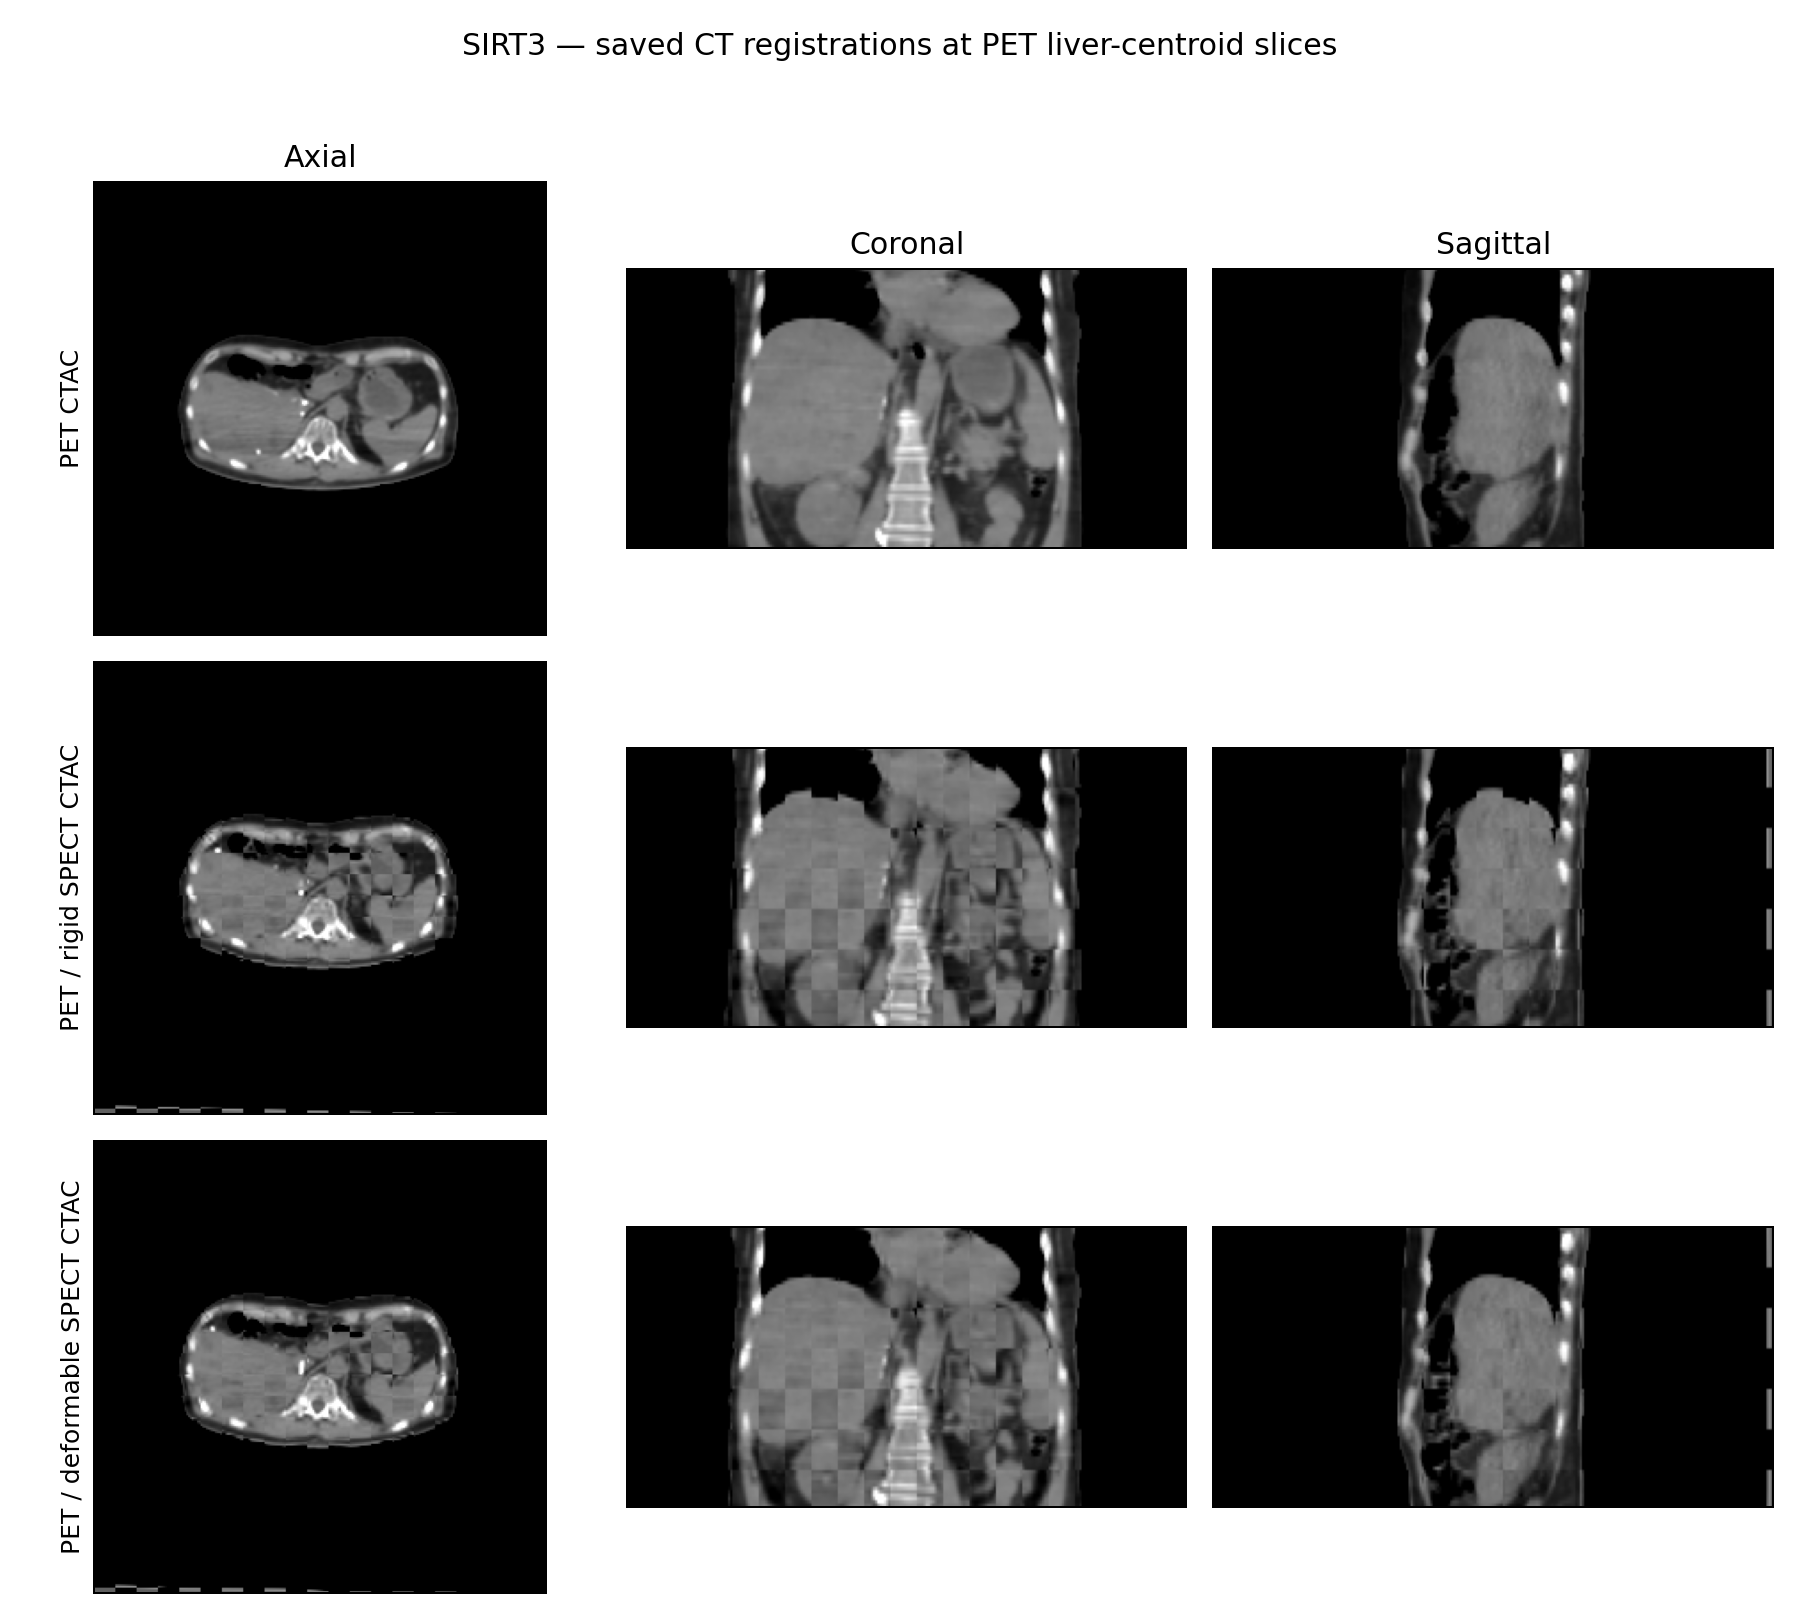
\includegraphics[width=0.9\linewidth,trim=0 0 0 0.5in,clip]{figures/Chapter6/patients/sirt3/registration_sirt3.png}
    \caption{PET/SPECT CTAC registration for the training patient (SIRT3), shown on axial, coronal and sagittal slices through the centroid of the liver segmented on the PET CTAC. Top: PET CTAC alone. Middle and bottom: checkerboards alternating the PET CTAC with the SPECT CTAC after rigid alignment (middle) and after deformable refinement (bottom), in 12-voxel blocks. All panels use the same slices and a $-150$ to $250$~\gls{hu} window, and voxel aspect ratios are respected. Anatomical continuity across block boundaries indicates alignment.}
    \label{fig:90y_registration_sirt3}
\end{figure}

\section{Data and evaluation protocol}
\label{sec:90y_data_eval}

All quantitative image analysis is performed on PET reconstructions to preserve direct comparability with SHKEM, where PET is the target modality and SPECT provides guidance. SPECT reconstructions are shown for completeness but are not included in the quantitative endpoints. Reconstruction hyperparameters are tuned once using the clinical training patient (SIRT3) and then fixed for all phantom and clinical reconstructions. This single-patient tuning strategy avoids repeated adjustment on the evaluation cohort, but it does not constitute a robustness study of the selected weights. Throughout, \dtv, \wtnv, and SHKEM are compared against the reference method \wdtnv.

\subsection{Phantom data}
\label{subsec:90y_phantom}

A \glsentryshort{nema} \glsentryshort{iec} Body Phantom with a sphere-to-background ratio of 8 was scanned at The Christie Hospital using a Siemens Biograph mCT PET/CT system and a GE Discovery 670 SPECT/CT system. \glsentryshort{pet} was acquired over \SI{15}{\hour} and \glsentryshort{spect} over \SI{15}{\minute}. From the \SI{15}{\hour} \glsentryshort{pet} acquisition, $N_{\mathrm{bs}}=20$ statistically independent \glsentryshort{pet} datasets equivalent to \SI{15}{\minute} were generated by sinogram bootstrapping \cite{markiewiczAssessmentBootstrapResampling2014}. The SPECT energy window was $39.84$--$128.16~\mathrm{keV}$.

We quantify \glsentryshort{pet} reproducibility across bootstraps via voxel-wise \acrfull{cov}, and \glsentryshort{pet} quantification via \acrfullpl{rc} for spheres of diameters \SI{10}{mm}, \SI{13}{mm}, \SI{22}{mm}, \SI{28}{mm}, and \SI{37}{mm}. Three \glspl{voi} were defined (Figure~\ref{fig:90y_nema_bootstrap_overview}): a high-count (HC) VOI comprising five filled spheres (one sphere was excluded due to filling issues), a warm-background (BG) VOI comprising the phantom volume excluding the spheres plus a \SI{10}{mm} margin and excluding the lung insert plus a \SI{5}{mm} margin, and the cold lung insert (LI).

\begin{figure}[htbp]
    \centering
    \begin{subfigure}[b]{0.39\linewidth}
        \centering
        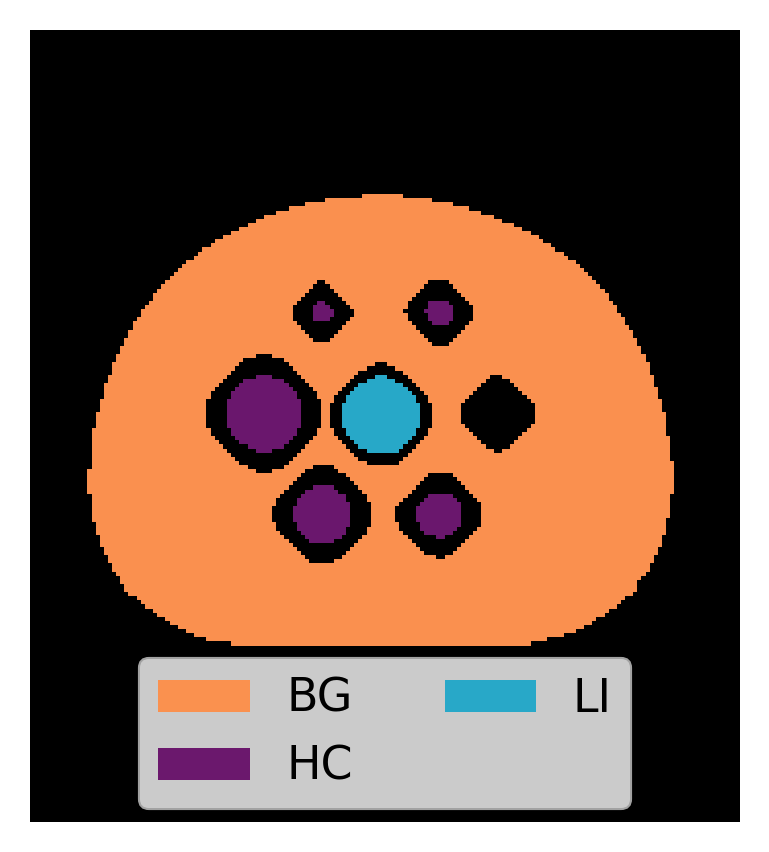
\includegraphics[width=\linewidth,trim=0 0 0 1.8in,clip]{figures/Chapter6/phantoms/manc_nema/bootstrap_mask.png}
    \end{subfigure}%
    \hfill
    \begin{subfigure}[b]{0.58\linewidth}
        \centering
        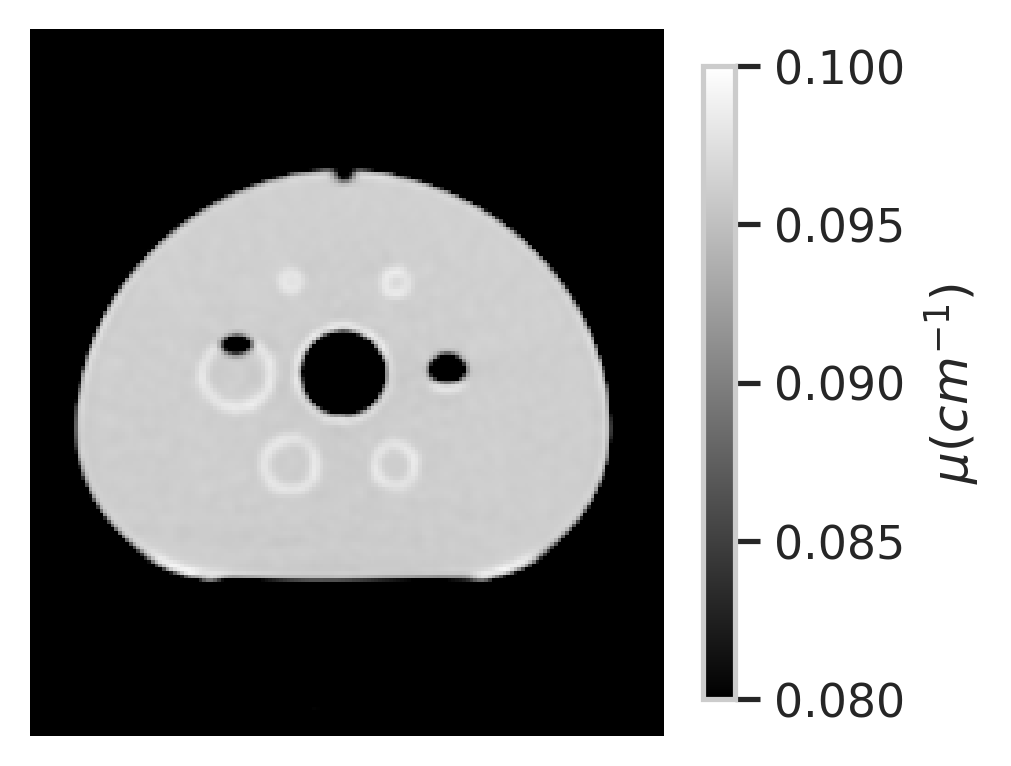
\includegraphics[width=\linewidth,trim=0 0 0 1.8in,clip]{figures/Chapter6/phantoms/manc_nema/bootstrap_umap.png}
    \end{subfigure}
    \caption{NEMA phantom analysis regions. Left: warm-background (BG), lung insert (LI), and high-count (HC) VOIs. Right: CTAC-derived attenuation map showing sphere edges, the lung insert, and the under-filled sphere excluded from the HC VOI.}
    \label{fig:90y_nema_bootstrap_overview}
\end{figure}

Let $z^{(c)}_{1,\mathrm{bs},n}$ be the reconstructed PET intensity at shared-grid voxel $n$ for method $c$ in bootstrap realisation $\mathrm{bs}\in\{1,\dots,N_{\mathrm{bs}}\}$. Define the inter-bootstrap mean and standard deviation
\begin{equation}
\bar z^{(c)}_{1,n} := \frac{1}{N_{\mathrm{bs}}}\sum_{\mathrm{bs}=1}^{N_{\mathrm{bs}}} z^{(c)}_{1,\mathrm{bs},n},
\qquad
\mathrm{SD}^{(c)}_n := \sqrt{\frac{\sum_{\mathrm{bs}=1}^{N_{\mathrm{bs}}}\left(z^{(c)}_{1,\mathrm{bs},n}-\bar z^{(c)}_{1,n}\right)^2}{N_{\mathrm{bs}}-1}},
\end{equation}
and voxel-wise
\begin{equation}
\mathrm{CoV}^{(c)}_n = \frac{\mathrm{SD}^{(c)}_n}{\bar z^{(c)}_{1,n}}.
\end{equation}
For a \glsentryshort{voi} $\mathcal{V}$ we report the \glsentryshort{voi}-averaged statistic
\begin{equation}
\overline{\mathrm{CoV}}^{(c)}_{\mathcal{V}}
=\frac{1}{|\mathcal{V}|}\sum_{n\in \mathcal{V}} \mathrm{CoV}^{(c)}_{n}.
\end{equation}

For sphere $v$, let $\bar{C}^{(c)}_{\mathrm{bs},v}$ denote the mean reconstructed intensity within the sphere and $\bar{C}^{(c)}_{\mathrm{bs},\mathrm{bkg}}$ the mean within BG for the same $(c,\mathrm{bs})$. With true ratio $R_{\mathrm{true}}=8$, define
\begin{equation}
\mathrm{RC}^{(c)}_{\mathrm{bs},v} = \frac{\bar{C}^{(c)}_{\mathrm{bs},v}}{\bar{C}^{(c)}_{\mathrm{bs},\mathrm{bkg}}\,R_{\mathrm{true}}}.
\end{equation}

To assess statistical significance of inter-bootstrap CoV, we compare each method $c$ with the reference $c_0=\wdtnv$ using a paired row-swap permutation test on $\log(\overline{\mathrm{CoV}}^{(c)}_{\mathcal{V}})$. Let $X^{(c)}_{\mathcal{V}}\in\mathbb{R}^{N_{\mathrm{bs}}\times|\mathcal{V}|}$ be the bootstrap-by-voxel stack restricted to VOI $\mathcal{V}$, and define the observed difference $d_{\mathrm{obs}}=\log(\overline{\mathrm{CoV}}^{(c_0)}_{\mathcal{V}})-\log(\overline{\mathrm{CoV}}^{(c)}_{\mathcal{V}})$. Under the null of exchangeability, each bootstrap index is independently swapped between the paired stacks with probability $1/2$ to form permuted differences $d_{\mathrm{perm}}$. We use $N_{\mathrm{perm}}=5000$ permutations and compute the two-sided p-value
\begin{equation}
p =
\frac{1+\sum_{i=1}^{N_{\mathrm{perm}}}\mathbf{1}\!\left(|d_{\mathrm{perm},i}|\ge |d_{\mathrm{obs}}|\right)}
{N_{\mathrm{perm}}+1},
\end{equation}
with \acrfull{bh} adjustment across methods within each VOI\@. No thresholding was applied to exclude near-zero voxels, so CoV estimates in the cold lung insert should be interpreted as a noise-realisation stability measure rather than a conventional percentage variability around a substantial mean signal.

We analyse log-transformed RC using a linear mixed-effects model with fixed effects for reconstruction method, sphere, and their interaction. A random intercept for each bootstrap replicate accounts for measurements obtained from the same resampled dataset. The interaction allows the method differences to vary with sphere size. The full model specification is given in Appendix~\ref{app:90y_statistical_models}.
For each sphere size, many-to-one contrasts compare each method to the reference $c_0=\wdtnv$, with Benjamini--Hochberg adjustment across planned comparisons within that sphere. Since the model is fitted on the log scale, $\exp(\Delta_{c,v})<1$ indicates lower recovery than \wdtnv for sphere $v$.

\subsection{Clinical data}
\label{subsec:90y_clinical}

Clinical data were acquired at Oxford University Hospitals from 10 patients undergoing $^{90}$Y \glsentryshort{sirt}: one patient was used for hyperparameter selection and nine for testing. \glsentryshort{pet} was acquired on a GE Discovery 710 PET/CT system and \glsentryshort{spect} on a GE Discovery NM/CT 670 system. Informed consent is not necessary for retrospective image reviews of this nature at Oxford University Hospitals. \glsentryshort{pet} was acquired with two bed positions (\SI{15}{\minute} each) and \glsentryshort{spect} over \SI{20}{\minute} on a dual-head system. Energy windows were $50$--$150~\mathrm{keV}$.

Tumour \glspl{voi} were delineated once per patient on the vendor Q.Clear
$\beta$-4000 \glsentryshort{pet} reconstruction using an adapted automatic
radial-gradient method based on Mikell \textit{et al.}
\cite{mikellImpact90YPET2018}. Candidate seed voxels were processed in
descending order of intensity, with a minimum seed separation of
\SI{30}{\milli\metre}. From each seed, the lesion boundary was estimated along
radial rays by the maximum image-gradient magnitude after Gaussian smoothing
($\sigma=0.1$); each ray was limited to a
maximum length of \SI{25}{\milli\metre} and a background-adjusted intensity
floor $I_{\mathrm{bkg}}+0.42(I_{\mathrm{seed}}-I_{\mathrm{bkg}})$, where
$I_{\mathrm{bkg}}$ is the mean intensity in the manually defined homogeneous
liver background \glsentryshort{voi}. The 42\% fraction was motivated by the
PET lesion-delineation thresholds reported by Erdi \textit{et al.}
\cite{erdiSegmentationLungLesion1997}. Masks containing fewer than 10 voxels
were discarded, and the five highest-ranked non-overlapping masks were
retained; where candidate masks overlapped, the mask originating from the
hotter seed took precedence. These \glspl{voi} were propagated unchanged
across all reconstructions so that measured differences reflected
reconstruction effects rather than \glsentryshort{voi} definition. The intensity
floor was a pragmatic search bound, not a validated threshold for
post-\glsentryshort{sirt} liver lesions; no delineation-accuracy or
parameter-sensitivity study was performed.

A homogeneous liver background \glsentryshort{voi} was drawn manually,
avoiding motion and visible artefacts. The training-patient lesion and
background \glspl{voi} are shown in Figure~\ref{fig:90y_sirt3_rois}.

\begin{figure}[htbp]
    \centering
    \begin{subfigure}[b]{0.32\linewidth}
        \centering
        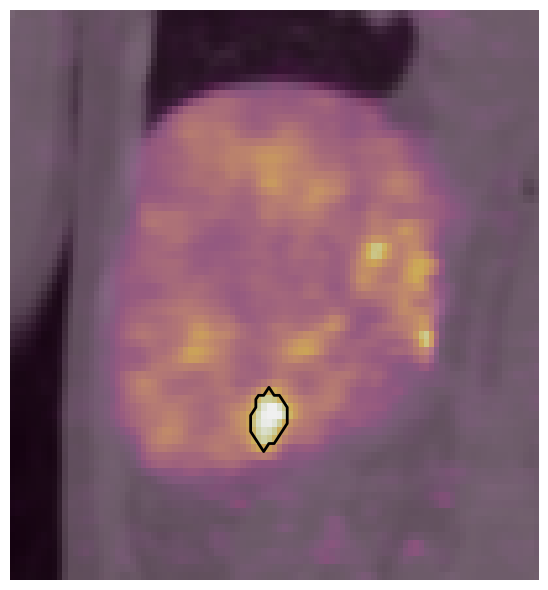
\includegraphics[width=\linewidth]{figures/Chapter6/patients/sirt3/lesion_1.png}
    \end{subfigure}%
    \hfill
    \begin{subfigure}[b]{0.32\linewidth}
        \centering
        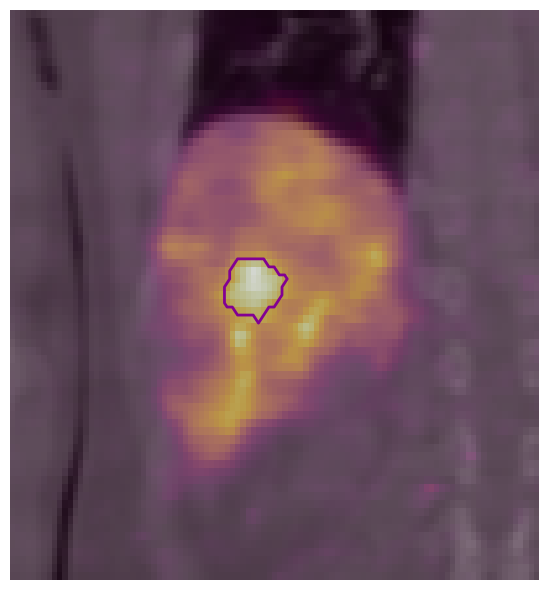
\includegraphics[width=\linewidth]{figures/Chapter6/patients/sirt3/lesion_2.png}
    \end{subfigure}%
    \hfill
    \begin{subfigure}[b]{0.32\linewidth}
        \centering
        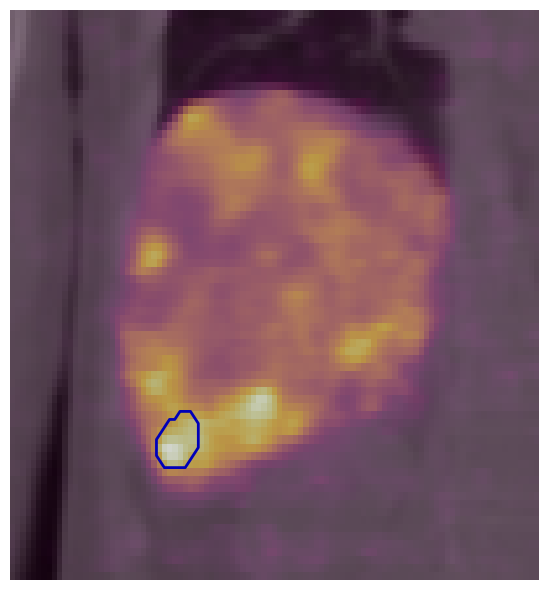
\includegraphics[width=\linewidth]{figures/Chapter6/patients/sirt3/lesion_3.png}
    \end{subfigure}%
    \vspace{-0.4cm}
    \begin{subfigure}[b]{0.32\linewidth}
        \centering
        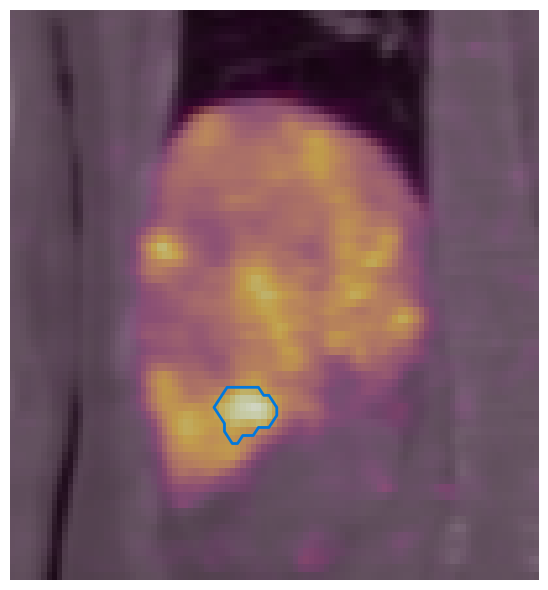
\includegraphics[width=\linewidth]{figures/Chapter6/patients/sirt3/lesion_4.png}
    \end{subfigure}
    \hfill
    \begin{subfigure}[b]{0.32\linewidth}
        \centering
        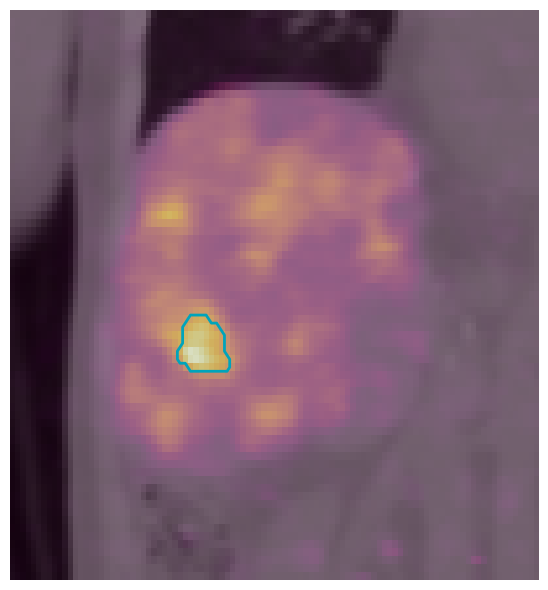
\includegraphics[width=\linewidth]{figures/Chapter6/patients/sirt3/lesion_5.png}
    \end{subfigure}%
    \hfill
    \begin{subfigure}[b]{0.32\linewidth}
        \centering
        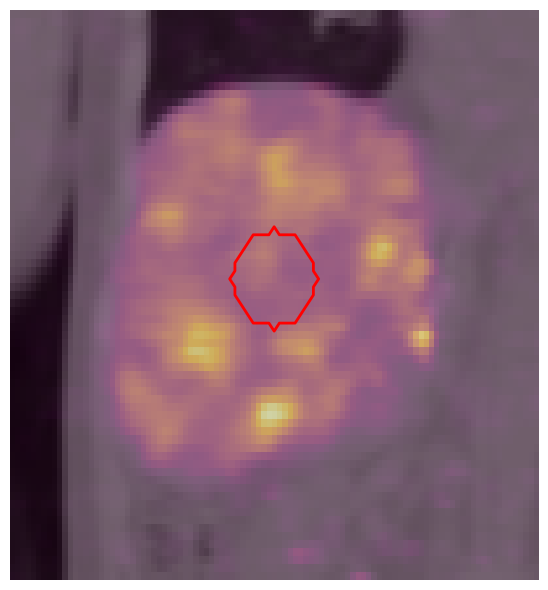
\includegraphics[width=\linewidth]{figures/Chapter6/patients/sirt3/background.png}
    \end{subfigure}
    \caption{Training-patient VOIs. The five identified lesions and the background reference region are shown on the vendor PET reconstruction with registered attenuation maps. Top row: lesions 1--3. Bottom row: lesions 4--5 and background.}
    \label{fig:90y_sirt3_rois}
\end{figure}

For patient $p$, lesion $l$, and method $c$, define \acrfull{tbr}
\begin{equation}
\mathrm{TBR}_{p,l,c}=\frac{\bar{C}_{p,l,c}}{\bar{C}_{p,\mathrm{bkg},c}},
\end{equation}
and background noise (percentage CoV)
\begin{equation}
\mathrm{CoV}_{p,c}(\%) = 100\,\frac{\mathrm{SD}_{p,c}}{\bar{C}_{p,\mathrm{bkg},c}},
\end{equation}
where $\mathrm{SD}_{p,c}$ is the within-background-VOI standard deviation.

We analyse log-transformed TBR using a linear mixed-effects model with a fixed effect for reconstruction method and random intercepts for patient and lesion within patient. These account for repeated measurements of the same lesion and for lesions belonging to the same patient. Log-transformed background CoV is analysed at the patient level, with a fixed method effect and a random patient intercept. Full model specifications are given in Appendix~\ref{app:90y_statistical_models}.
Planned many-to-one contrasts compare \dtv, \wtnv, and SHKEM to \wdtnv using two-sided Wald $z$-tests, with \glsentryshort{bh} adjustment across the three comparisons within each endpoint. Results are reported as ratios $\exp(\Delta)$ on the original scale, where values below one indicate lower TBR or lower background CoV than \wdtnv.

\section{Results}
\label{sec:90y_results}

\subsection{Hyperparameter selection}
\label{subsec:90y_hyperparams}

Regularisation weights $\beta_{\mathrm{PET}}$ and $\beta_{\mathrm{SPECT}}$ in \eqref{eq:90y_rhom_def} were tuned on a single training patient by sweeping the TBR--$\mathrm{CoV}_{\mathrm{bkg}}$ trade-off and identifying the Pareto frontier: settings where neither higher TBR nor lower background CoV could be obtained without worsening the other. From these settings, we selected an operating point with background CoV approximately matched to the vendor reconstruction. The selected weights were then fixed for all phantom and clinical experiments:
\begin{table}[htbp]
\centering
\caption{Selected regularisation weights (tuned on a single training patient) used for all phantom and clinical experiments.}
\label{tab:90y_hyperparams}
\small
\begin{tabular}{lcc}
\toprule
\textbf{Method} & $\boldsymbol{\beta_{\mathrm{PET}}}$ & $\boldsymbol{\beta_{\mathrm{SPECT}}}$ \\
\midrule
\wdtnv & 0.01   & 0.02 \\
\wtnv  & 0.0075 & 0.02 \\
\dtv   & 0.02   & -- \\
\bottomrule
\end{tabular}
\end{table}

For SHKEM, hyperparameters followed Deidda \textit{et al.} \cite{deiddaTripleModalityImage2023}; the PET subiteration displayed and analysed here (27) was chosen to approximately match the background CoV of the vendor reconstruction.

Figure~\ref{fig:90y_tradeoff} shows the training-patient trade-off curves for two representative lesions. Lesion~1 shows only a modest initial benefit from synergistic information and is largely insensitive to further increases in SPECT weighting until over-regularisation introduces negative bias. Lesion~2 shows a clearer synergistic benefit: increasing SPECT weighting shifts the TBR--$\mathrm{CoV}_{\mathrm{bkg}}$ curve towards higher TBR at comparable background CoV up to a distinct elbow region, after which excessive coupling reduces TBR and/or increases background CoV. For lesion~2, the PET image obtained with \wdtnv also exhibited features consistent with a CTAC artefact; this is discussed in Section~\ref{sec:90y_discussion}.

\begin{figure*}[htbp]
    \centering
    \begin{subfigure}[b]{\textwidth}
        \centering
        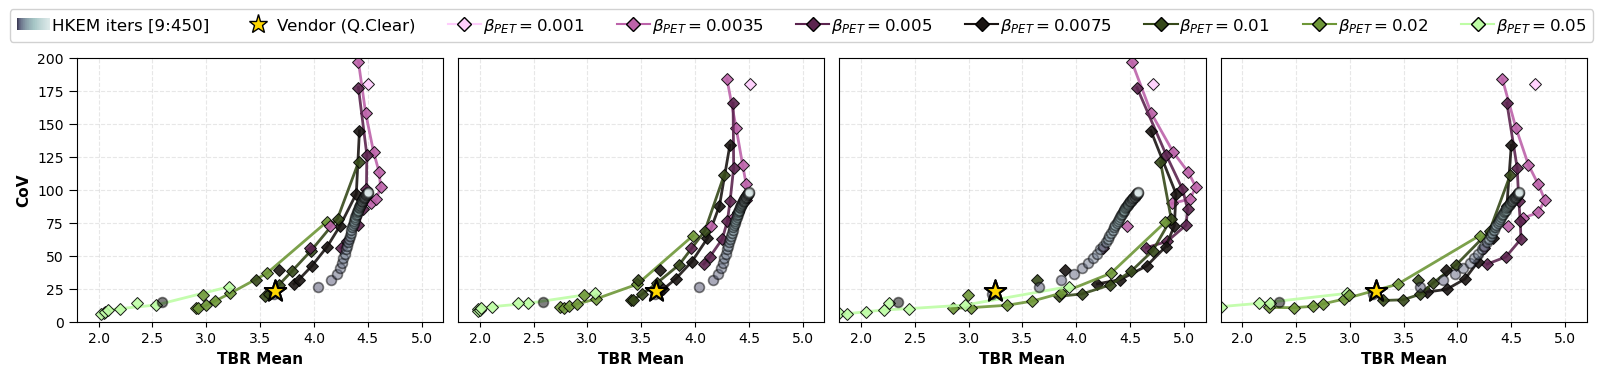
\includegraphics[width=\linewidth]{figures/Chapter6/patients/sirt3/lesion_1_2_constant_pet.png}
    \vspace{-0.5cm}
    \end{subfigure}
    \begin{subfigure}[b]{\textwidth}
        \centering
        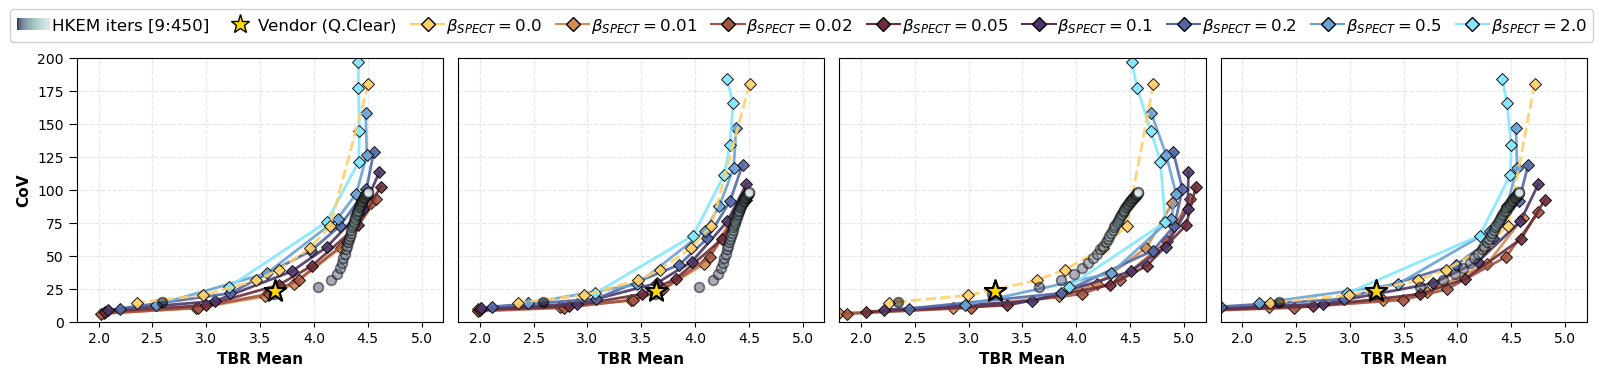
\includegraphics[width=\linewidth]{figures/Chapter6/patients/sirt3/lesion_1_2_constant_spect.png}
    \end{subfigure}
    \caption{Training-patient hyperparameter sweep. Impact of varying SPECT weighting while holding PET regularisation constant (top row) and varying PET weighting while holding SPECT regularisation constant (bottom row) on TBR and $\mathrm{CoV}_{\mathrm{bkg}}$ for lesions 1 and 2. The first and third columns show \wdtnv; the second and fourth show \wtnv.}
    \label{fig:90y_tradeoff}
\end{figure*}

\subsection{Phantom results}
\label{subsec:90y_phantom_results}

A representative reconstruction from a single bootstrapped PET realisation is shown in Figure~\ref{fig:90y_phantom_recon_comparison} (PET and corresponding SPECT; for SHKEM, SPECT is the separately reconstructed guidance image; \dtv does not reconstruct SPECT).
\begin{figure}[htbp]
    \centering
    \begin{subfigure}[b]{0.99\linewidth}
        \centering
        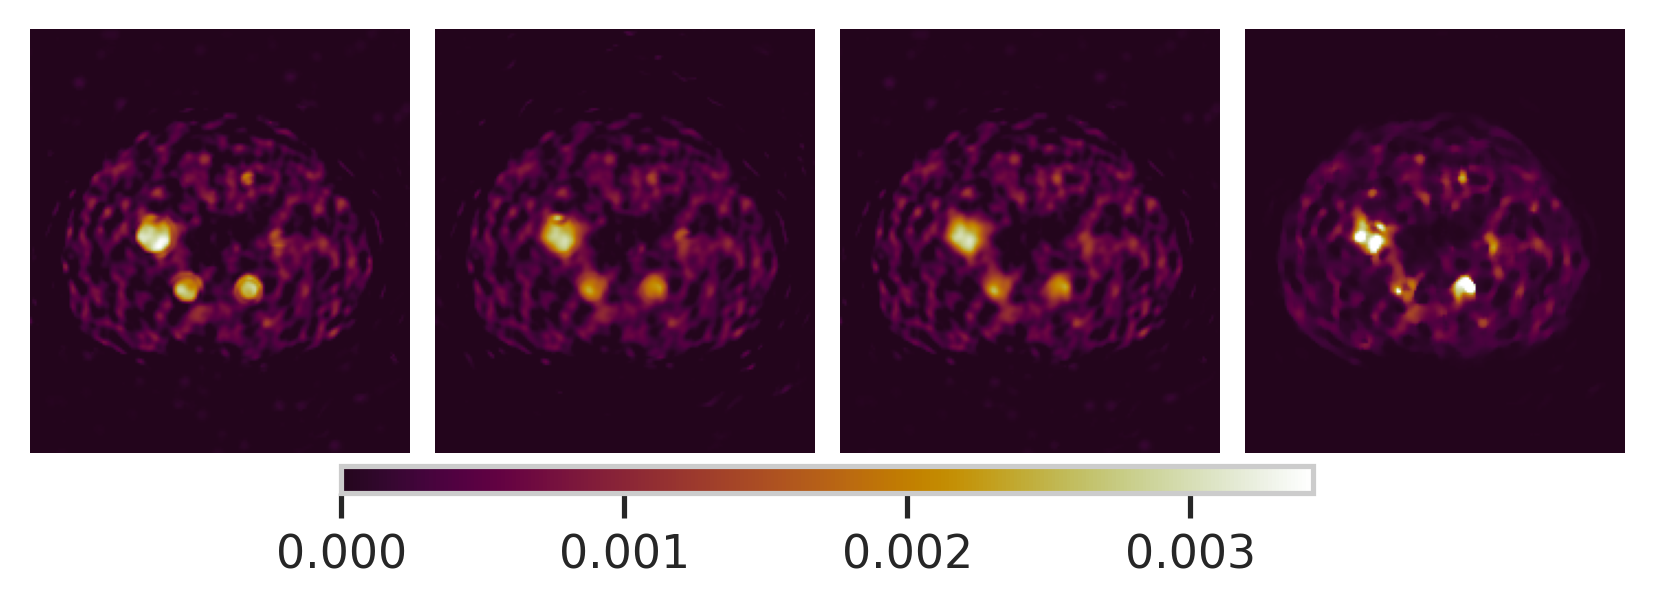
\includegraphics[width=\linewidth]{figures/Chapter6/phantoms/manc_nema/bootstrap_random_pet.png}
    \end{subfigure}
    \vspace{-0.5cm}
    \begin{subfigure}[b]{0.99\linewidth}
        \centering
        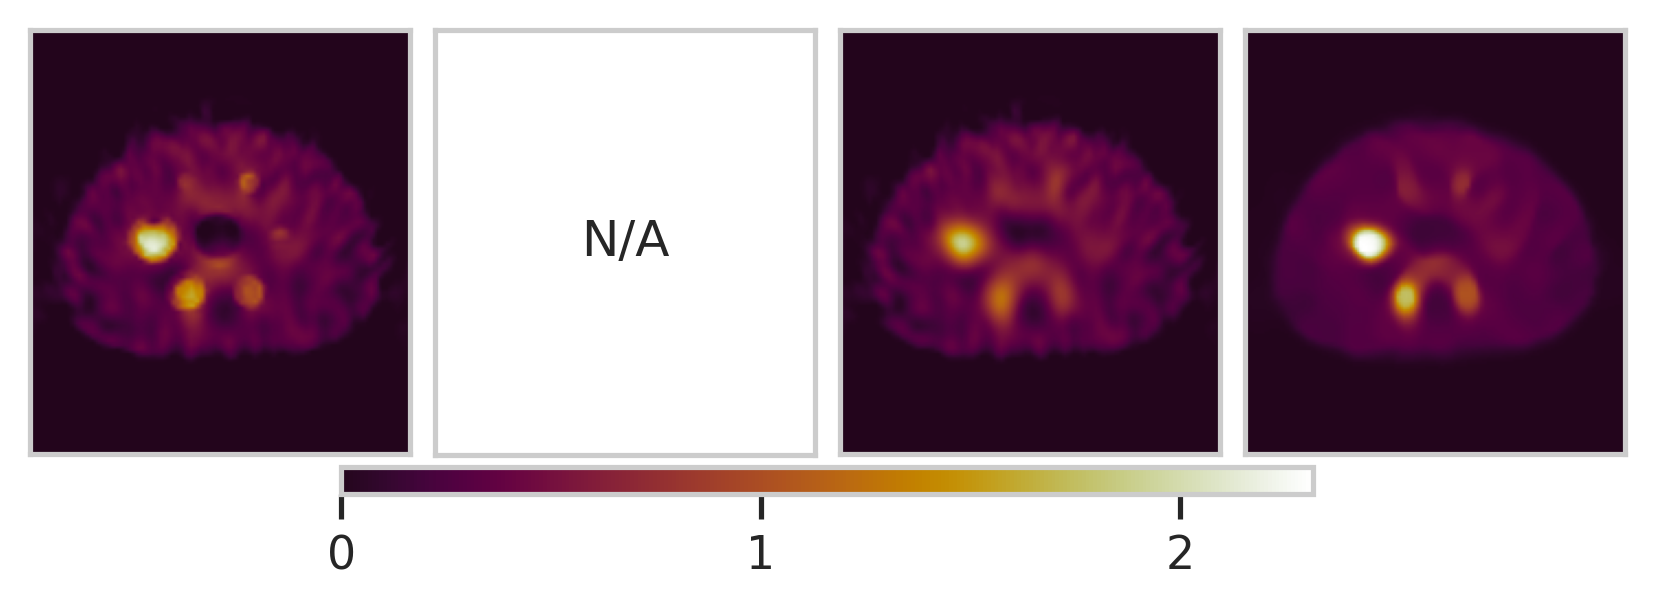
\includegraphics[width=\linewidth]{figures/Chapter6/phantoms/manc_nema/bootstrap_random_spect.png}
    \end{subfigure}
    \caption{Visual comparison of NEMA phantom reconstructions for a randomly chosen bootstrap. From left to right: \wdtnv, \dtv, \wtnv, SHKEM (subiteration 27). PET reconstructions are shown on the top row and SPECT on the bottom row (SPECT guidance for SHKEM). Images are displayed in reconstruction intensity units, proportional to activity concentration.}
    \label{fig:90y_phantom_recon_comparison}
\end{figure}

Figure~\ref{fig:90y_rc_spheres_comparison} and Table~\ref{tab:90y_effect_ratio_rc} summarise sphere recovery. Quantitative analysis demonstrated that \wdtnv achieved significantly higher recovery than \dtv and \wtnv for all sphere sizes $\leq\SI{22}{\milli\metre}$. \wdtnv showed similar recovery to SHKEM in the larger spheres but significantly improved recovery for the two smallest spheres at the matched operating point.
\begin{figure*}[htbp]
    \centering
    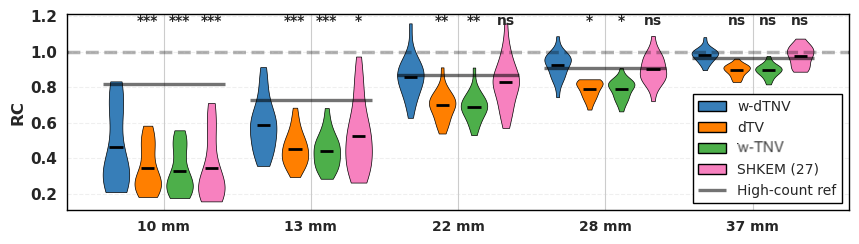
\includegraphics[width=\linewidth]{figures/Chapter6/phantoms/manc_nema/bootstrap_rc.png}
    \caption{Recovery coefficient (RC) for NEMA phantom spheres for \wdtnv, \dtv, \wtnv and SHKEM (subiteration 27). Also shown are the equivalent RCs for a high-count, long-OSEM reconstruction. The grey line indicates perfect recovery. Statistical significance is reported for paired comparisons versus \wdtnv (Benjamini--Hochberg adjusted): $^*$ $p<0.05$, $^{**}$ $p<0.01$, $^{***}$ $p<0.001$.}
    \label{fig:90y_rc_spheres_comparison}
\end{figure*}

\begin{table}[htbp]
\centering
\footnotesize
\setlength{\tabcolsep}{5pt}
\begin{tabular}{l l c l l}
\toprule
Method & $v$ & $\exp(\Delta_{c,v})$ & 95\% CI & $p_{\mathrm{BH}}$ \\
\midrule
\dtv & 37\,mm & 0.9113 & [0.8001,\,1.0380] & 0.2472 \\
     & 28\,mm & 0.8543 & [0.7500,\,0.9730] & 0.0267 \\
     & 22\,mm & 0.8165 & [0.7168,\,0.9300] & 0.0034 \\
     & 13\,mm & 0.7819 & [0.6865,\,0.8906] & 0.00043\\
     & 10\,mm & 0.7706 & [0.6766,\,0.8777] & $<10^{-4}$ \\
\addlinespace
\wtnv & 37\,mm & 0.9108 & [0.7997,\,1.0374] & 0.2472 \\
      & 28\,mm & 0.8544 & [0.7502,\,0.9732] & 0.0267 \\
      & 22\,mm & 0.8090 & [0.7103,\,0.9215] & 0.0034 \\
      & 13\,mm & 0.7598 & [0.6671,\,0.8654] & 0.0001 \\
      & 10\,mm & 0.7384 & [0.6483,\,0.8410] & $<10^{-4}$ \\
\addlinespace
SHKEM (27) & 37\,mm & 0.9931 & [0.8720,\,1.1312] & 0.9175 \\
           & 28\,mm & 0.9739 & [0.8551,\,1.1093] & 0.6906 \\
           & 22\,mm & 0.9616 & [0.8443,\,1.0953] & 0.5559 \\
           & 13\,mm & 0.8723 & [0.7659,\,0.9936] & 0.0397 \\
           & 10\,mm & 0.7381 & [0.6480,\,0.8407] & $<10^{-4}$ \\
\bottomrule
\end{tabular}
\caption{Effect ratios $\exp(\Delta_{c,v})$ (comparator vs.\ baseline \wdtnv) with 95\% confidence intervals and BH-adjusted $p$-values, reported by sphere diameter $v$. Values below one indicate lower recovery coefficient than \wdtnv.}
\label{tab:90y_effect_ratio_rc}
\end{table}

Figure~\ref{fig:90y_phantom_cov} summarises voxel-wise reproducibility across bootstraps. At the matched operating point, \dtv and \wtnv yield lower voxel-wise CoV than \wdtnv in the evaluated VOIs, consistent with stronger effective smoothing. SHKEM exhibits higher variability in background and high-count regions but improved stability in the cold lung insert. Sphere-level CoV trends were consistent with the voxel-wise analysis, with \wtnv and \dtv generally providing the lowest variability across the evaluated sphere diameters and SHKEM the highest.
\begin{figure}[htbp]
    \centering
    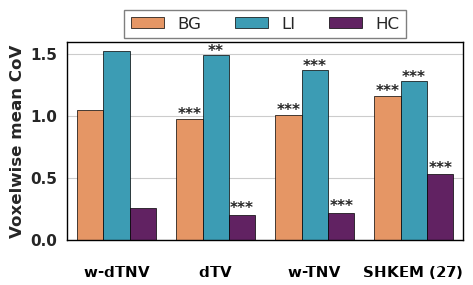
\includegraphics[width=\linewidth]{figures/Chapter6/phantoms/manc_nema/bootstrap_voxelwise_cov.png}
    \caption{VOI-mean inter-bootstrap voxel coefficient of variation (CoV, dimensionless ratio) across 20 bootstrapped PET realisations within each VOI\@. The groups from left to right are \wdtnv, \dtv, \wtnv and SHKEM (27). Statistical significance is reported for paired comparisons versus \wdtnv (BH-adjusted): $^*$ $p<0.05$, $^{**}$ $p<0.01$, $^{***}$ $p<0.001$.}
    \label{fig:90y_phantom_cov}
\end{figure}

\subsection{Clinical results}
\label{subsec:90y_clinical_results}

Figure~\ref{fig:90y_sirt3_visuals} shows representative PET and SPECT reconstructions for the training patient. These images illustrate the operating-point behaviour used to select the fixed regularisation weights: \wdtnv improves lesion contrast where the SPECT and CTAC-derived guidance contain useful structural information, while the response is weaker where there is no clear anatomical correlate.

\begin{figure*}[hbtp]
    \centering
    \begin{minipage}[htbp]{0.49\textwidth}
        \centering
        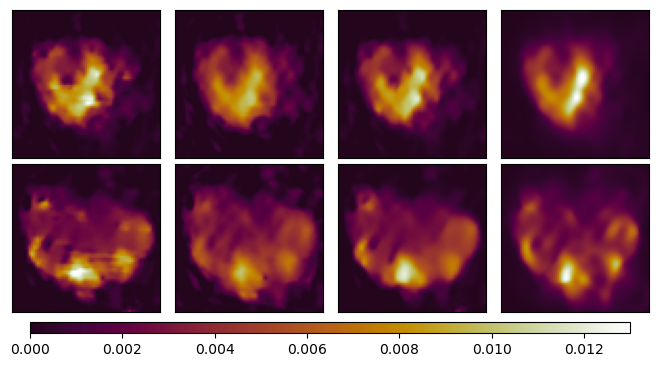
\includegraphics[width=\linewidth]{figures/Chapter6/patients/sirt3/recons/pet_axial.png}\par
        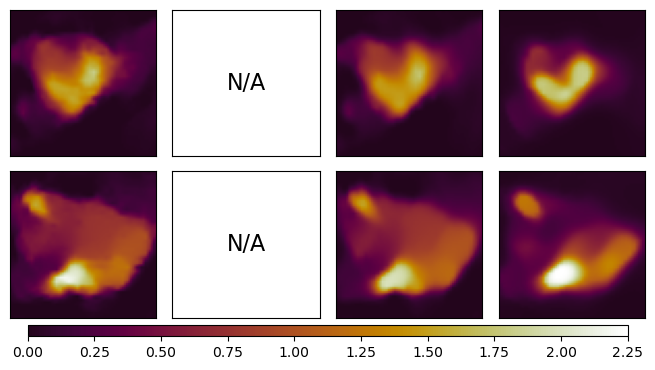
\includegraphics[width=\linewidth]{figures/Chapter6/patients/sirt3/recons/spect_axial.png}\par
        \textbf{Axial views}.
    \end{minipage}\hfill
    \begin{minipage}[htbp]{0.49\textwidth}
        \centering
        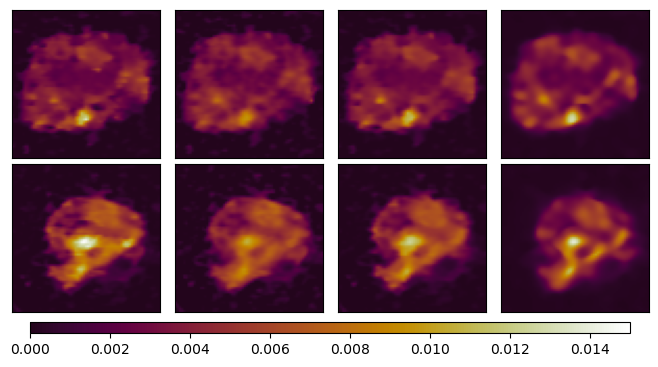
\includegraphics[width=\linewidth]{figures/Chapter6/patients/sirt3/recons/pet_coronal.png}\par
        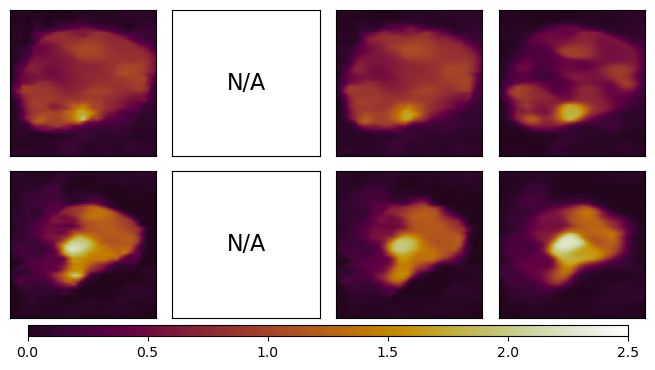
\includegraphics[width=\linewidth]{figures/Chapter6/patients/sirt3/recons/spect_coronal.png}\par
        \textbf{Coronal views}.
    \end{minipage}
    \caption{Visual comparison of reconstruction methods for training patient SIRT3. Columns show \wdtnv, \dtv, \wtnv and SHKEM (subiteration 27). The upper two quadrants show PET reconstructions; the lower two show SPECT reconstructions or guidance images. Images are displayed in reconstruction intensity units, proportional to activity concentration.}
    \label{fig:90y_sirt3_visuals}
\end{figure*}

Across the test cohort, \wdtnv yields higher lesion TBR than \dtv, \wtnv, and SHKEM at the matched operating point, while background CoV differences are smaller and method-dependent. SHKEM reconstructions appeared visually smoother and, as in the phantom, appeared more effective at suppressing cold-background noise:
\begin{figure}[htbp]
    \centering
    \begin{subfigure}[b]{0.49\linewidth}
        \centering
        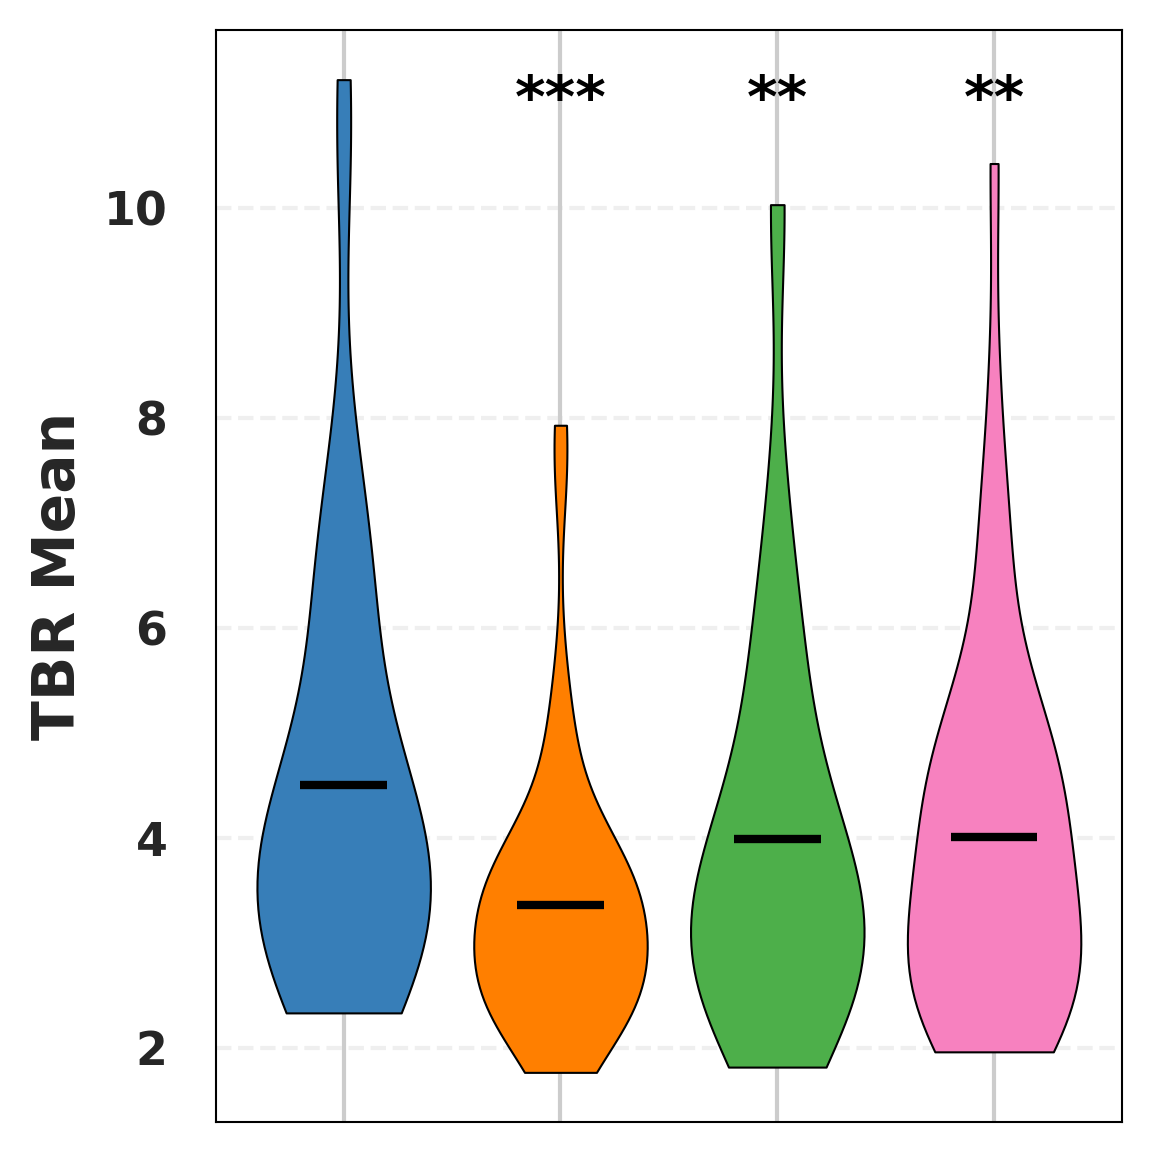
\includegraphics[width=\linewidth]{figures/Chapter6/patients/all_lesions_tbr_mean.png}
    \end{subfigure}%
    \hfill
    \begin{subfigure}[b]{0.49\linewidth}
        \centering
        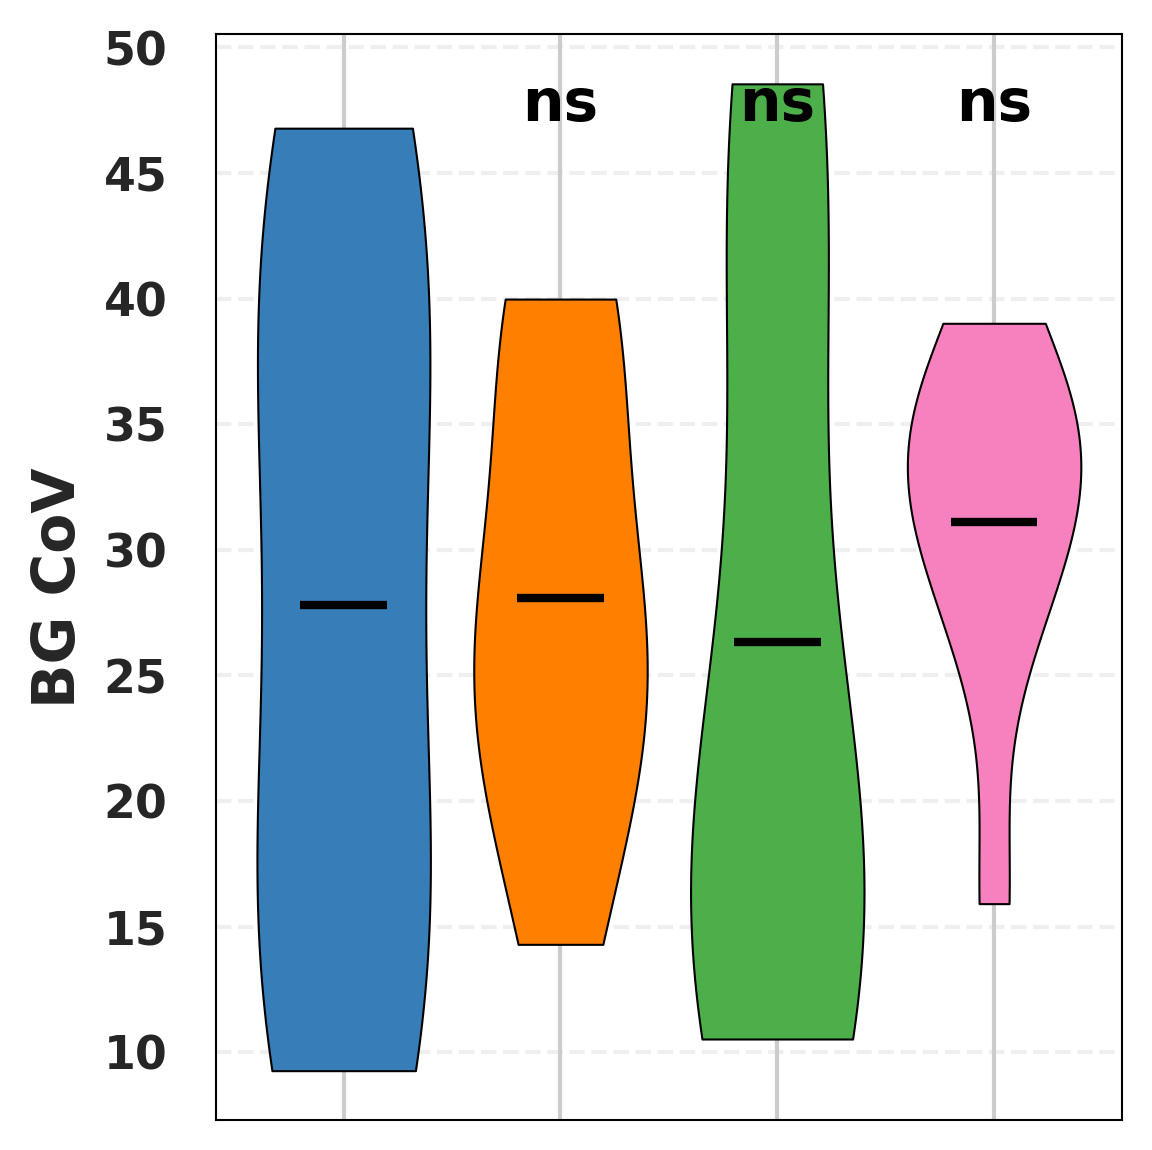
\includegraphics[width=\linewidth]{figures/Chapter6/patients/all_lesions_bg_cov.png}
    \end{subfigure}%
    \caption{Clinical cohort summary: lesion-wise mean TBR (left) and patient-wise spatial background CoV (percentage, right). In both panels, methods from left to right are \wdtnv, \dtv, \wtnv and SHKEM (27); black lines mark means. Statistical significance is reported for comparisons versus \wdtnv (BH-adjusted): $^*$ $p<0.05$, $^{**}$ $p<0.01$, $^{***}$ $p<0.001$.}
    \label{fig:90y_patient_summary}
\end{figure}

\begin{table}[htbp]
\centering
\footnotesize
\setlength{\tabcolsep}{5pt}
\begin{tabular}{l c l l}
\toprule
Method & $\exp(\Delta)$ & 95\% CI & $p_{\mathrm{BH}}$ \\
\midrule
\dtv        & 0.803 & [0.763,\,0.845] & $1.26\times10^{-16}$ \\
\wtnv       & 0.918 & [0.872,\,0.966] & 0.00153 \\
SHKEM (27)  & 0.930 & [0.884,\,0.979] & 0.00560 \\
\bottomrule
\end{tabular}
\caption{Effect ratios $\exp(\Delta)$ with 95\% Wald confidence intervals and BH-adjusted $p$-values for mean tumour-to-background ratio (TBR), comparing each method to \wdtnv. Values below one indicate lower TBR than \wdtnv.}
\label{tab:90y_effect_ratio_tb}
\end{table}

\begin{table}[htbp]
\centering
\footnotesize
\setlength{\tabcolsep}{5pt}
\begin{tabular}{l c l l}
\toprule
Method & $\exp(\Delta)$ & 95\% CI & $p_{\mathrm{BH}}$ \\
\midrule
\dtv        & 1.183 & [0.903,\,1.549] & 0.334 \\
\wtnv       & 1.008 & [0.769,\,1.320] & 0.956 \\
SHKEM (27)  & 1.339 & [1.022,\,1.753] & 0.103 \\
\bottomrule
\end{tabular}
\caption{Effect ratios $\exp(\Delta)$ with 95\% Wald confidence intervals and BH-adjusted $p$-values for background CoV, comparing each method to \wdtnv. Values above one indicate higher background CoV than \wdtnv.}
\label{tab:90y_effect_ratio_cov}
\end{table}

\section{Discussion}
\label{sec:90y_discussion}

At the matched operating point, \wtnv alone did not recover the smallest sphere boundaries. Adding anatomical guidance, explicitly in \wdtnv or implicitly through CT-informed SHKEM features, improved boundary localisation. The gain of \wdtnv over \wtnv and \dtv was largest for the smallest spheres, where PET counts and SPECT resolution were most limiting.

At the selected operating point, \dtv and \wtnv had lower voxel-wise CoV than \wdtnv, suggesting stronger effective smoothing. The variational methods were more repeatable than SHKEM in background and high-count regions, while SHKEM was most stable in the cold lung insert. One possible explanation is that its kernel weights average nearby near-zero voxels, so positivity reinforces the cold region. This may improve stability there without improving repeatability elsewhere.

\dtv and \wtnv produced broadly similar PET appearances in the phantom, despite \dtv including $\mu$-directional guidance and \wtnv including PET/SPECT coupling. In this experiment, then, neither CTAC-derived directional guidance alone nor isotropic PET/SPECT coupling alone was sufficient to recover the smallest structures. The improved recovery with \wdtnv points to a complementary mechanism: the higher-count SPECT image provides additional functional support for the location of activity transitions, while the $\mu$-derived directional field reduces penalisation of gradients aligned with anatomical boundaries.

The lesion results were not uniform. Lesions with clear anatomical correlates, such as calcification or liver-capsule boundaries visible in the $\mu$-map, tended to benefit more from directional guidance and PET/SPECT coupling. Lesions without a corresponding anatomical structure showed less improvement. This is consistent with the design of \wdtnv: CTAC guidance changes the preferred edge directions without directly prescribing emission intensities, but it can still bias reconstructed structure.

For example, lesion 2 in the training patient shows substantial improvement in the TBR--CoV trade-off as SPECT weighting is increased (Figure~\ref{fig:90y_tradeoff}). Post-hoc examination indicates that this lesion lies adjacent to a calcified region visible in the $\mu$-map, providing a sharp anatomical edge that coincides with the functional boundary. Lesion 3 also improves under both \wdtnv and \wtnv; this lesion abuts the liver on three sides, where the soft-tissue interface generates reasonably strong anatomical contrast. For \wdtnv, the $\mu$-map liver boundary provides explicit directional guidance aligned with the functional uptake margin, while for \wtnv the SPECT boundary may be sufficiently well defined to support PET/SPECT coupling even without directional CTAC guidance.

Conversely, lesion 1 shows little benefit from increasing SPECT weighting until excessive weighting introduces negative bias. Visual inspection shows no obvious anatomical correlate at the tumour margin, and the PET and SPECT images appear already well aligned. The reason for this lesion's limited response to synergistic reconstruction remains unclear.

One practical limitation is sensitivity to CTAC artefacts. Because $\xi_n$ depends on $D\mu$, streaks can enter $\|\xi\|$ and then the reconstructed emission images. In the training patient, arms-down acquisition introduced streaking and beam-hardening artefacts in the PET CTAC. The stabiliser $\eta$ suppresses amplification of small gradients but not necessarily coherent, high-contrast artefacts. SHKEM used a SPECT attenuation map acquired with arms raised, so its guidance input differed from the one used by \wdtnv; this may explain why streak-related artefacts were less apparent in SHKEM.

\begin{figure*}[t]
    \centering
    \begin{minipage}[t]{0.49\textwidth}
        \centering
        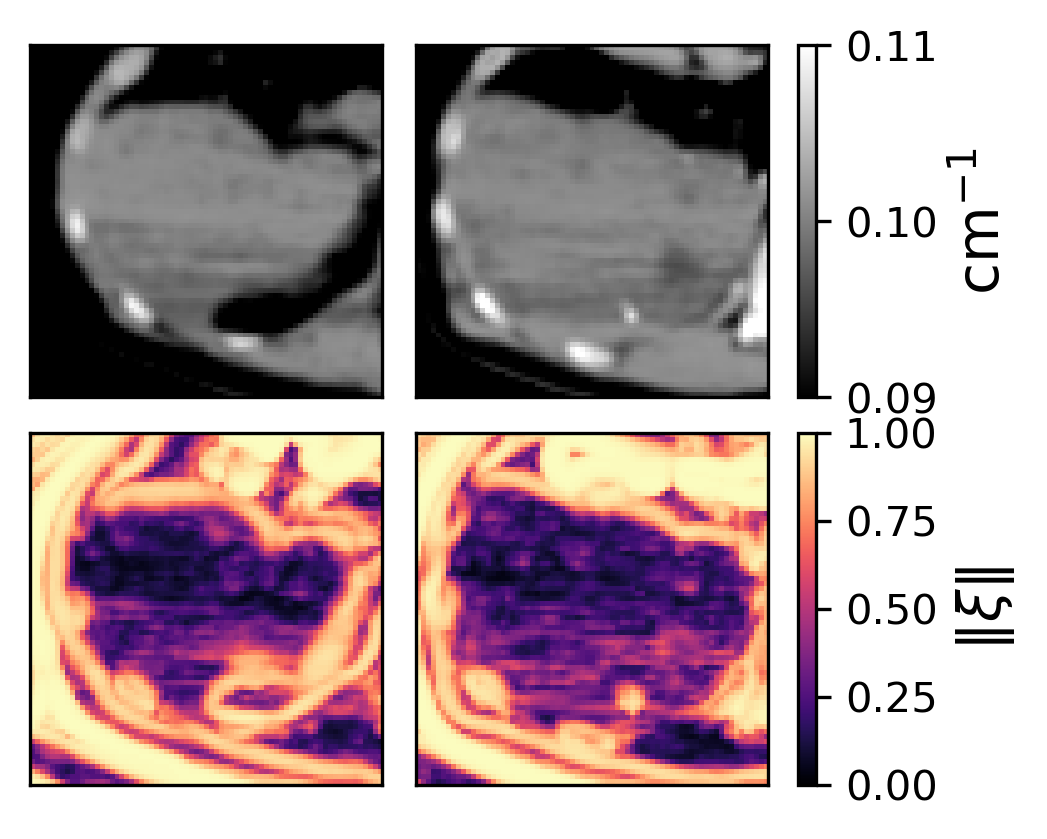
\includegraphics[width=\linewidth]{figures/Chapter6/patients/sirt3/axial_ddiff.png}\par
        \textbf{Axial slice}.
    \end{minipage}\hfill
    \begin{minipage}[t]{0.49\textwidth}
        \centering
        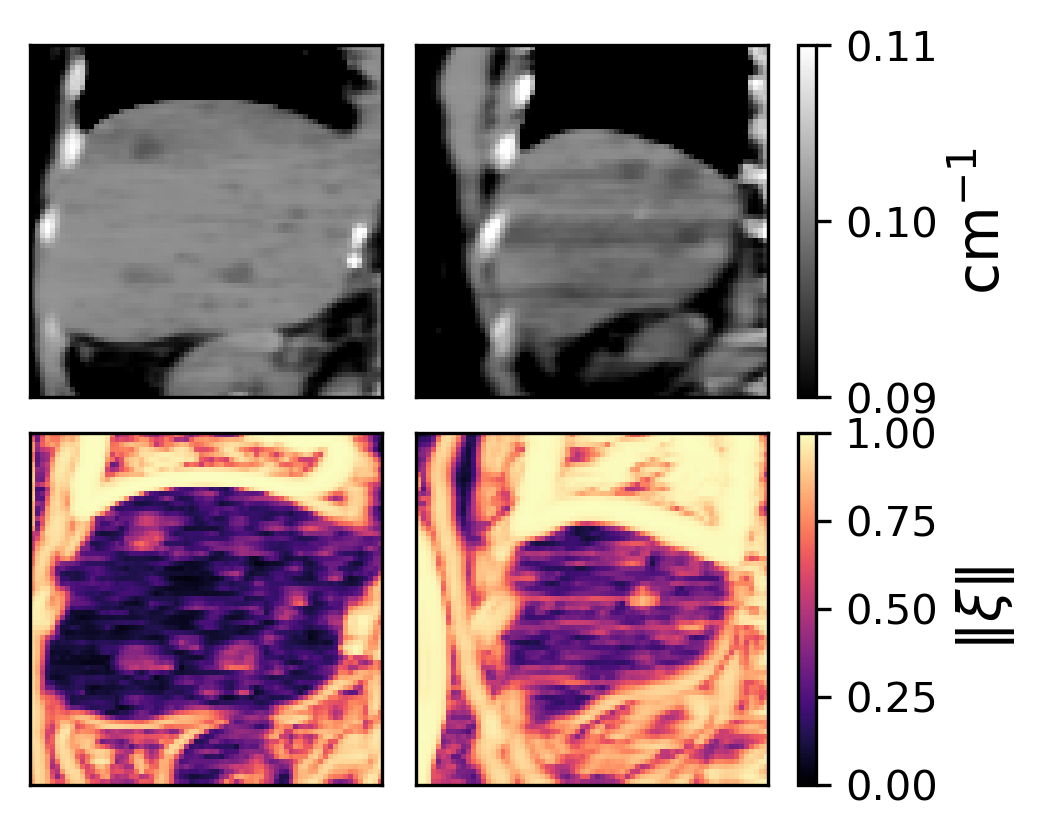
\includegraphics[width=\linewidth]{figures/Chapter6/patients/sirt3/coronal_ddiff.png}\par
        \textbf{Coronal slice}.
    \end{minipage}
    \caption{Training-patient CTAC-derived guidance. The CTAC-derived attenuation map $\mu$ (top row; cm$^{-1}$) and magnitude of the \wdtnv directional weighting field $\|\xi\|$ (bottom row) are shown for lesions 1 and 2. CTAC streak artefacts are visible in $\mu$ and are reproduced in $\|\xi\|$, providing a pathway for artefact transfer into the emission reconstruction.}
    \label{fig:90y_patient_ctac_xi}
\end{figure*}

The contrast with the NEMA phantom is instructive (Figure~\ref{fig:90y_nema_ctac_xi}). In the phantom, the CTAC is largely free of coherent streak artefacts and the resulting $\|\xi\|$ follows the true boundaries and insert edges. In this setting, directional smoothing reduced small high-frequency fluctuations without visible CT-related artefacts in the displayed reconstruction.

\begin{figure}[hbtp]
    \centering
    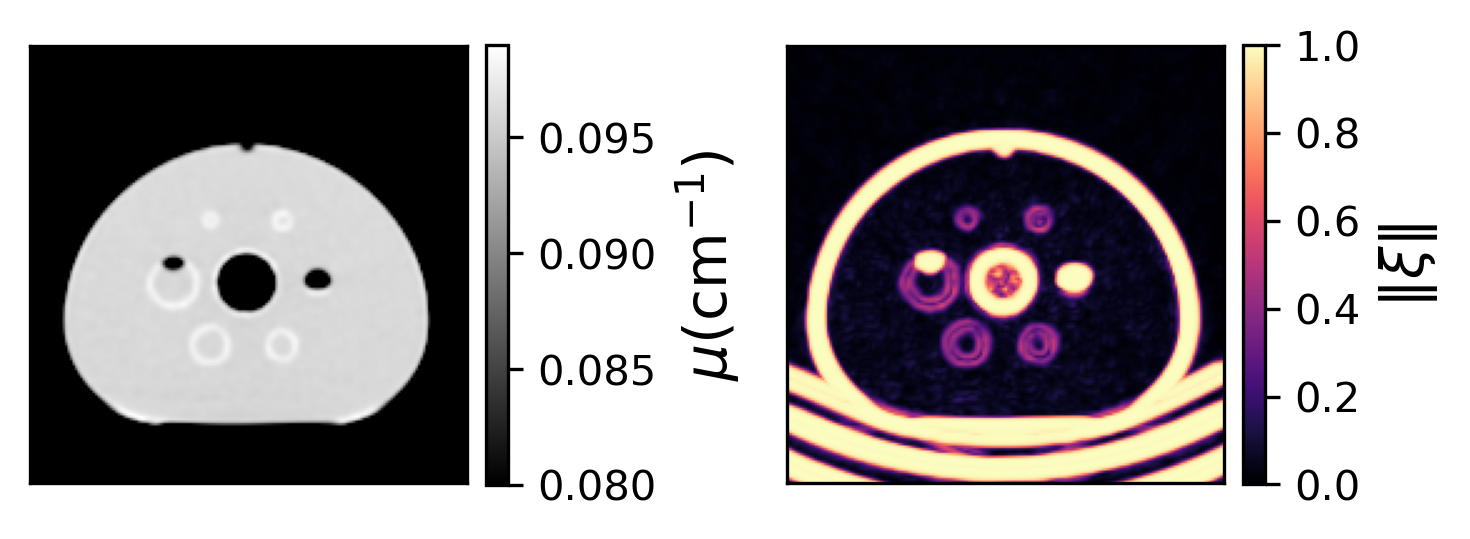
\includegraphics[width=\linewidth]{figures/Chapter6/phantoms/manc_nema/axial_ddiff.png}
    \caption{NEMA phantom, central axial slice. CTAC-derived attenuation map $\mu$ (left; cm$^{-1}$) and magnitude of the \wdtnv directional weighting field $\|\xi\|$ (right). With a high-quality CTAC free of prominent streak artefacts, $\|\xi\|$ concentrates around true object boundaries and insert edges, enabling stable $\mu$-map-guided directional smoothing.}
    \label{fig:90y_nema_ctac_xi}
\end{figure}

These observations motivate future work on robust direction-field estimation and artefact-aware guidance strategies. From a practical perspective, if a low-dose CTAC is used to provide directional information, acquisition protocols that minimise artefacts, such as arms raised where feasible, are preferable.

To preserve direct comparability with SHKEM, regularisation weights were selected once on the clinical training case and quantitative evaluation focused on PET\@. How well these weights transfer to other acquisition protocols and lesion presentations was therefore not established. The jointly reconstructed SPECT images were assessed qualitatively only. Although they appeared less noisy while maintaining lesion conspicuity, a rigorous assessment of SPECT quantification would require modality-specific lesion delineation and evaluation protocols. The sensitivity of \wdtnv to residual PET/SPECT/CT registration error was likewise not characterised.

More broadly, this chapter focuses on the favourable case in which PET and SPECT image the same underlying $^{90}$Y microsphere distribution. The same framework may be extendable to settings with non-identical functional distributions but shared anatomy, such as planning--treatment image pairs ($^{99\mathrm{m}}$Tc-MAA versus post-treatment $^{90}$Y), multi-nuclide imaging, or multi-timepoint studies. In such cases, the directional/anatomical component remains well motivated, but the inter-modality coupling strength may need to be relaxed or made spatially adaptive to avoid transferring modality-specific or temporally evolving uptake features.

\section{Conclusion}
\label{sec:90y_conclusion}

This chapter validated the $w$-$d$TNV prior of Chapter~\ref{chapter:wdtnv} in joint $^{90}$Y PET/SPECT reconstruction with CTAC-derived directional guidance. The single-bed optimisation framework of Chapter~\ref{chapter:optimisation} was extended to reconstruct the patient PET bed positions jointly, allowing the prior to act across the combined field of view. The qualitative comparison in Figure~\ref{fig:optim_multibed_qualitative} showed overlap-region noise and discontinuities after independent reconstruction and fusion that were not apparent in the joint multi-bed example. The key modelling choice is to use CTAC information directionally (via $\Pi_{m,n}$) while preserving a two-modality Jacobian, retaining the computational advantages of the $2\times 2$ Gram structure (Chapter~\ref{chapter:wdtnv}) and avoiding unstable intensity coupling to CT.

On a bootstrapped NEMA IEC phantom, \wdtnv improves small-object recovery relative to \wtnv, \dtv, and a sequential hybrid kernel baseline at a matched noise operating point, with significant gains over the isotropic and non-synergistic variational baselines. Repeatability is better than SHKEM in the background and high-count regions, although it is lower than for the more strongly smoothing \wtnv and \dtv baselines; SHKEM remains most stable in the cold lung insert. In the post-SIRT cohort of 45 lesions across nine patients, \wdtnv yields significantly higher lesion TBR than the comparators at approximately matched background CoV. The response is not uniform across lesions. Those with clear anatomical correlates, such as calcification or liver boundaries, benefit most from synergy and $\mu$-map-informed edge alignment, while lesions without corresponding anatomical structure show less improvement. These findings support CTAC-guided synergistic variational coupling as a way to improve post-SIRT $^{90}$Y activity imaging for personalised dosimetry, but clinical translation will depend on controlling CT artefacts and PET/SPECT/CT registration error.

\SA{Well done on presenting such a lot of complex information. It's dense but it's followable. I am sure this will be fine in a viva although there might be a lot of questions.}
